%documentclass{buthesis}          %Gives author-year citation style
\documentclass[numbib, twoadv]{buthesis} %Gives numerical citation style
%\documentclass[twoadv}{buthesis} %Allows entry of second advisor
%\usepackage{graphics}            %Select graphics package
\usepackage{graphicx}             %
\usepackage{pdfpages}             %For including PDF pages in appendices
%\usepackage{amsthm}              %Add other packages as necessary
\usepackage{array}                %Extended column types and \arraybackslash
\usepackage{makecell}             %Multi-line table header cells
\usepackage{tabularx}             %Auto-width table columns
\usepackage{tikz}                 %For programmatic diagrams
\usetikzlibrary{shapes,arrows,positioning,fit,backgrounds,decorations.pathreplacing}
\usepackage[
    hidelinks,
    linktoc=all,
    pdfpagemode=UseOutlines
]{hyperref}  %Enable hyperlinks and PDF bookmarks
\hyphenation{HRIStudio}
\begin{document}
\butitle{A Web-Based Wizard-of-Oz Platform for Collaborative and Reproducible Human-Robot Interaction Research}
\author{Sean O'Connor}
\degree{Bachelor of Science}
\department{Computer Science}
\advisor{L. Felipe Perrone}
\advisorb{Brian King}
\chair{Alan Marchiori}
\maketitle

\frontmatter

\acknowledgments{
    (Draft Acknowledgments)
}

\tableofcontents

\listoftables

\listoffigures

\abstract{
    The Wizard-of-Oz (WoZ) technique is widely used in Human-Robot Interaction (HRI) research to prototype and evaluate robot interaction designs before autonomous capabilities are fully developed. However, two persistent problems limit the technique's effectiveness. First, existing WoZ tools impose high technical barriers that prevent domain experts outside engineering from conducting independent studies (the Accessibility Problem). Second, the fragmented landscape of custom, robot-specific tools makes it difficult to verify or replicate experimental results across labs (the Reproducibility Problem). This thesis formalizes a set of design principles for WoZ infrastructure that address both problems simultaneously: a hierarchical specification model that organizes experiments as studies, experiments, steps, and actions; an event-driven execution model that separates protocol design from live trial control; and a plugin architecture that decouples experiment logic from robot-specific implementations. These principles are realized in HRIStudio, an open-source, web-based platform that provides a visual experiment designer, a guided wizard execution interface, automated timestamped logging with explicit deviation tracking, and role-based access control for research teams. A pilot between-subjects study compared HRIStudio against Choregraphe, a representative baseline tool, using six faculty participants who each designed and executed an interactive storytelling task on a NAO robot. Across all six sessions, HRIStudio participants achieved higher design fidelity (mean 100 vs. 56.7), higher execution reliability (mean 96.7 vs. 66.7), and higher perceived usability (mean SUS 76.7 vs. 59.2) than Choregraphe participants. The only unprompted specification deviation in the dataset occurred in the Choregraphe condition, illustrating the reproducibility failure mode HRIStudio's enforcement model is designed to prevent. While the pilot scale precludes inferential claims, the directional evidence across all measures suggests that the right software architecture can make WoZ experiments more accessible to non-programmers and more reproducible across executions.
}

\mainmatter

\chapter{Introduction}
\label{ch:intro}

\section{Motivation}

To build the social robots of tomorrow, researchers must find ways to convincingly simulate them today. The process of designing and optimizing interactions between human and robot is essential to the field of Human-Robot Interaction (HRI), a discipline dedicated to ensuring these technologies are safe, effective, and accepted by the public. However, current practices for prototyping these interactions are often hindered by complex technical requirements and inconsistent methodologies.

In a typical social robotics interaction, a robot operates autonomously based on pre-programmed behaviors. Because human interaction is inherently unpredictable, pre-programmed autonomy often fails to respond appropriately to subtle social cues, causing the interaction to degrade. To overcome this, researchers utilize the Wizard-of-Oz (WoZ) technique, where a human operator--the ``wizard''--controls the robot's actions in real-time, creating the illusion of autonomy. This allows for rapid prototyping and testing of interaction designs before the underlying artificial intelligence is fully matured.

Despite its versaility, WoZ research faces two critical challenges. First, a high technical barrier prevents many non-programmers, such as experts in psychology or sociology, from conducting their own studies without engineering support. Second, the hardware landscape is highly fragmented. Researchers frequently build bespoke, ``one-off'' control interfaces for specific robots and specific experiments. These ad-hoc tools are rarely shared, making it difficult for the scientific community to replicate studies or verify findings. This has led to a replication crisis in HRI, where a lack of standardized tooling undermines the reliability of the field's body of knowledge.

\section{HRIStudio Overview}

To address these challenges, this thesis presents HRIStudio, a web-based platform designed to manage the entire lifecycle of a WoZ experiment: from interaction design, through live execution, to final analysis.

HRIStudio is built on three core design principles: disciplinary accessibility, scientific reproducibility, and platform sustainability. To achieve accessibility, the platform replaces complex code with a visual, drag-and-drop interface, allowing domain experts to design interaction flows much like creating a storyboard. To ensure reproducibility, HRIStudio enforces a structured experimental workflow that acts as a ``smart co-pilot'' for the wizard. It guides them through a standardized script to minimize human error while automatically logging synchronized data streams for analysis. Finally, unlike tools tightly coupled to specific hardware, HRIStudio utilizes a robot-agnostic architecture to ensure sustainability. This design ensures that the platform remains a viable tool for the community even as individual robot platforms become obsolete.

\section{Research Objectives}

The primary objective of this work is to demonstrate that a unified, web-based software framework can significantly improve both the accessibility and reproducibility of HRI research. Specifically, this thesis aims to develop a production-ready platform, validate its accessibility for non-programmers, and assess its impact on experimental rigor.

First, this work translates the foundational architecture proposed in prior publications into a stable, full-featured software platform capable of supporting real-world experiments. Second, through a formal user study, we evaluate whether HRIStudio allows participants with no robotics experience to successfully design and execute a robot interaction, comparing their performance against industry-standard software. Finally, we quantify the impact of the platform's guided execution features on the consistency of wizard behavior and the accuracy of data collection.

This work builds upon preliminary concepts reported in two peer-reviewed publications \cite{OConnor2024, OConnor2025}. It extends that research by delivering the complete implementation of the system and a comprehensive empirical evaluation of its efficacy.

\chapter{Background and Context}
\label{ch:background}

\section{Human-Robot Interaction and Wizard-of-Oz}
% TODO

HRI is a multidisciplinary field dedicated to understanding, designing, and evaluating robotic systems for use by or with humans. Unlike industrial robotics, where safety often means physical separation, social robotics envisions a future where robots operate in shared spaces, collaborating with people in roles ranging from healthcare assistants and educational tutors to customer service agents.

For these interactions to be effective, robots must exhibit social intelligence. They must recognize and respond to human social cues--such as speech, gaze, and gesture--in a manner that is natural and intuitive. However, developing the artificial intelligence required for fully autonomous social interaction is an immense technical challenge. Perception systems often struggle in noisy environments, and natural language understanding remains an area of active research.

To bridge the gap between current technical limitations and desired interaction capabilities, researchers employ the WoZ technique. In a WoZ experiment, a human operator (the ``wizard'') remotely controls the robot's behaviors, unaware to the study participant. To the participant, the robot appears to be acting autonomously. This methodology allows researchers to test hypotheses about human responses to robot behaviors without needing to solve the underlying engineering challenges first.

\section{Prior Work}

This thesis represents the culmination of a multi-year research effort to address critical infrastructure gaps in the HRI community. The ideas presented here build upon a foundational trajectory established through two peer-reviewed publications.

We first introduced the concept for HRIStudio as a Late-Breaking Report at the 2024 IEEE International Conference on Robot and Human Interactive Communication (RO-MAN) \cite{OConnor2024}. In that work, we identified the lack of accessible tooling as a primary barrier to entry in HRI and proposed the high-level vision of a web-based, collaborative platform. We established the core requirements for the system: disciplinary accessibility, robot agnosticism, and reproducibility.

Following the initial proposal, we published the detailed system architecture and preliminary prototype as a full paper at RO-MAN 2025 \cite{OConnor2025}. That publication validated the technical feasibility of our web-based approach, detailing the communication protocols and data models necessary to support real-time robot control using standard web technologies.

While those prior publications established the ``what'' and the ``how'' of HRIStudio, this thesis focuses on the realization and validation of the platform. We extend our previous research in two key ways. First, we move beyond prototypes to deliver a complete, production-ready software platform (v1.0), resolving complex engineering challenges related to stability, latency, and deployment. Second, and crucially, we provide the first rigorous user study of the platform. By comparing HRIStudio against industry-standard tools, this work provides empirical evidence to support our claims of improved accessibility and experimental consistency.

\chapter{Reproducibility Challenges}
\label{ch:reproducibility}

Having established the landscape of existing WoZ platforms and their limitations, I now examine the factors that make WoZ experiments difficult to reproduce consistently and how software infrastructure can address them. This chapter analyzes the sources of variability identified in the WoZ literature and examines how current practices in infrastructure and reporting contribute to \emph{the Reproducibility Problem}. Understanding these challenges is essential for designing a system that supports reproducible, rigorous experimentation.

\section{Sources of Variability}

\emph{The Reproducibility Problem}, as introduced in Chapter~\ref{ch:intro}, encompasses two related challenges. The first concerns \emph{execution consistency}: whether a wizard reliably follows the same experimental script across multiple trials with different participants, producing comparable robot behavior in each. The second concerns \emph{cross-platform reproducibility}: whether the same experiment can be transferred to a different robot platform with minimal change to the implementing program. Both stem from gaps in current WoZ infrastructure and are examined in this chapter. A third interpretation of the term — independent replication of a published study by researchers at other institutions — is distinct from both and is not what this thesis evaluates. It is also worth noting that execution consistency, as defined here, corresponds to what the measurement literature sometimes calls \emph{repeatability}: the degree to which the same procedure produces consistent results when repeated across multiple trials of the same study.

In WoZ-based HRI studies, multiple sources of variability can compromise execution consistency. The wizard is simultaneously the strength and weakness of the WoZ paradigm. While human control enables sophisticated, adaptive interactions, it also introduces inconsistency. Consider a wizard conducting multiple trials of the same experiment with different participants.
 Even with a detailed script, the wizard may vary in timing, with delays between a participant's action and the robot's response fluctuating based on the wizard's attention, fatigue, or interpretation of when to act. When a script allows for choices, different wizards may make different selections, or the same wizard may act differently across trials. Furthermore, a wizard may accidentally skip steps, trigger actions in the wrong order, or misinterpret experimental protocols.

Riek's systematic review \cite{Riek2012} found that very few published studies reported measuring wizard error rates or providing standardized wizard training. Without such measures, it becomes impossible to determine whether experimental results reflect the intended interaction design or inadvertent variations in wizard behavior.

Beyond wizard behavior, the custom nature of many WoZ control systems introduces technical variability. When each research group builds custom software for each study, several problems arise. Custom interfaces may have undocumented capabilities, hidden features, default behaviors, or timing characteristics researchers never formally describe. Software tightly coupled to specific robot models or operating system versions may become unusable when hardware or software is upgraded or replaced. Each system logs data differently, with different file formats, different levels of granularity, and different choices about what to record. This fragmentation undermines both execution consistency and reproducibility. Rebuilding custom infrastructure for each study makes it nearly impossible to guarantee that wizard behavior is controlled the same way across trials. More broadly, reproducing the same experiment on a different robot platform typically requires reverse-engineering or rebuilding the original software from scratch.

Even when researchers intend for their work to be reproducible, practical constraints on publication length lead to incomplete documentation. Papers often omit exact timing parameters. Authors leave decision rules for wizard actions unspecified and fail to report details of the wizard interface. Specifications of data collection, including which sensor streams were recorded and at what sampling rate, frequently go missing. Without this information, other researchers cannot faithfully recreate the experimental conditions, limiting both direct replication and conceptual extensions of prior work.

\section{Infrastructure Requirements for Enhanced Reproducibility}

Based on this analysis, I identify specific ways that software infrastructure can mitigate reproducibility challenges:

\begin{enumerate}
\item \textbf{Guided wizard execution.} Rather than merely providing tools for wizard control, an ideal WoZ platform should actively guide wizards through scripted procedures. This means presenting actions in a prescribed sequence to prevent out-of-order execution, highlighting the current step in the protocol, recording any deviations from the script as explicit events in the data log, and supporting repeatable decision logic through clearly defined conditional branches. By constraining wizard behavior within the bounds of the experimental design, the system reduces unintended variability across trials and participants.

\item \textbf{Comprehensive automatic logging.} Manual data collection is error-prone and often incomplete. The platform should automatically record every action triggered by the wizard with precise timestamps, all robot sensor data and state changes, and timing information indicating when actions were requested, when they began executing, and when they completed. The full experimental protocol should be embedded in each log file so that researchers can recover the exact script used for any session. Note that recording precise timestamps does not imply that trials must have identical timing, since human-robot interactions naturally vary in duration; rather, the system captures what actually occurred for later analysis.

\item \textbf{Self-documenting protocol specifications.} The protocol specification itself should serve as documentation. When interaction protocols are defined using structured formats such as visual flowcharts or declarative scripts rather than imperative code, they become simultaneously executable and human-readable. Researchers can then share complete, unambiguous descriptions of their experimental procedures alongside their results.

\item \textbf{Platform-independent abstractions.} To maximize the lifespan and transferability of experimental designs, the platform must separate the high-level control logic, the sequence of wizard and robot actions, from the low-level details of how specific robots execute those behaviors. This abstraction allows experiments designed for one robot to be more easily adapted to another, extending the reproducibility of interaction designs even when the original hardware becomes obsolete.
\end{enumerate}



\section{Connecting Reproducibility Challenges to Infrastructure Requirements}

The reproducibility challenges identified above directly motivate the infrastructure requirements (R1--R6) established in Chapter~\ref{ch:background}. Inconsistent wizard behavior creates the need for real-time control mechanisms (R3) that guide wizards step by step, and for automatic logging (R4) that captures any deviations that occur. Timing errors further motivate responsive, fine-grained real-time control (R3): a wizard working with a sluggish interface introduces latency that disrupts the interaction and confounds timing analysis. Technical fragmentation forces each lab to rebuild infrastructure as hardware changes, violating platform agnosticism (R5). Incomplete documentation reflects the need for self-documenting, code-free protocol specifications (R2) that are simultaneously executable and shareable, integrated into a single workflow (R1) so that the specification and the execution environment are never separated. Finally, the isolation of individual research groups motivates collaborative support (R6): allowing multiple team members to observe and review trials enables the shared scrutiny that reproducibility requires. As Chapter~\ref{ch:background} demonstrated, no existing platform simultaneously satisfies all six requirements. Addressing this gap requires rethinking how WoZ infrastructure is designed, prioritizing reproducibility and methodological rigor as first-class design goals rather than afterthoughts.

\section{Chapter Summary}

This chapter has analyzed the reproducibility challenges inherent in WoZ-based HRI research, identifying three primary sources of variability: inconsistent wizard behavior, fragmented technical infrastructure, and incomplete documentation. Rather than treating these challenges as inherent to the WoZ paradigm, I showed how each stems from gaps in current infrastructure. Software design can systematically mitigate them through enforced experimental protocols, comprehensive automatic logging, self-documenting experiment designs, and platform-independent abstractions. These design goals directly address the six infrastructure requirements identified in Chapter~\ref{ch:background}. The following chapters describe the design, implementation, and pilot validation of a system that prioritizes reproducibility as a foundational design principle from inception.

\chapter{System Design}
\label{ch:design}

The previous chapters established the motivation for a web-based WoZ platform and identified six critical requirements for modern HRI research infrastructure. This chapter describes the design of HRIStudio, focusing on how the system architecture and experimental workflow implement these requirements. In this chapter I go over three key design decisions: the hierarchical structure of experiment specifications, the modular interface architecture, and the data flow during experiment execution.

\section{Hierarchical Organization of Experiments}

To address the need for self-documenting, executable experiment specifications (R1, R2), HRIStudio introduces a hierarchical organization of elements that allows researchers to express WoZ studies at multiple levels of abstraction. This structure enables experiment designs to be simultaneously intuitive for researchers to create and precise enough for the system to execute.

At the top level, researchers create a \emph{study} element that defines the overall research context, including metadata about the experiment, collaborators, and experimental conditions. A study comprises multiple \emph{experiment} elements, each representing a single session with one human subject using one robot configuration. This separation of study from experiment allows researchers to manage multiple instantiations of the same protocol while maintaining clear traceability.

Each experiment comprises a sequence of \emph{step} elements, which model distinct phases of the interaction. For example, an experiment might have steps such as ``Introduction,'' ``Learning Task,'' and ``Closing.'' Within each step, researchers define one or more \emph{action} elements that are the atomic units of the experimental procedure. Actions can be directed at the wizard (e.g., ``Wait for subject to finish task, then say encouraging phrase'') or at the robot (e.g., ``Move arm to point, play audio greeting, wait for subject response''). 

This hierarchical structure serves multiple purposes. First, it permits researchers to design experiments without programming knowledge, using visual or declarative specifications at each level. Second, it naturally maps to the temporal structure of the experimental session, making the protocol easy to follow during execution. Third, it provides a foundation for comprehensive logging: each action executed during a session can be recorded with precise timestamps and outcomes, making the experimental trace reproducible and analyzable.

\section{Modular Interface Architecture}

To support different roles in an experiment while maintaining coherent data flow (R3, R4, R6), HRIStudio implements three primary user interfaces, each optimized for a specific phase of the research lifecycle.

\subsection{Design Interface}

The \emph{Design} interface enables researchers to construct experiment specifications using drag-and-drop visual programming. Rather than requiring researchers to write code or complex configuration files, the interface presents a canvas where researchers can assemble pre-built action components into sequences. Components represent common tasks such as robot movements, speech synthesis, wizard instructions, and conditional logic. Researchers configure each component's parameters through property panels that provide contextual guidance and examples of best practices.

By treating experiment design as a visual specification task, the interface lowers technical barriers (R2) and ensures that the resulting protocol specification is human-readable and shareable alongside research results. The specification is stored in a structured, machine-readable format that can be both displayed as a flowchart and executed by the platform's runtime.

\subsection{Execute Interface}

During live experiment sessions, the system presents synchronized but distinct views to the wizard and observers. The \emph{wizard's Execute view} displays the current step and available actions, guiding the wizard through the experimental protocol while allowing flexibility for spontaneous, contextual responses. Actions are presented sequentially, but the wizard can manually trigger specific actions based on participant responses, ensuring that the interaction remains natural and responsive rather than rigidly scripted.

The wizard's view includes manual controls for unscripted behaviors such as additional robot movements, speech, or gestures. These unscripted actions are recorded in the experimental log as explicit deviations from the protocol, enabling researchers to later analyze both scripted and improvised interactions. This design balances the need for consistent, monitored behavior (which supports reproducibility) with the flexibility required for realistic human-robot interactions.

The \emph{observer's Execute view} enables additional researchers to monitor the experiment in real-time, take notes, and observe participant behavior without interfering with the wizard's control or the participant's experience. Multiple observers can simultaneously access this view, supporting collaborative oversight and interdisciplinary observation (R6).

\subsection{Analysis Interface}

After a live experiment session, the \emph{Analysis} interface enables researchers to review all recorded data streams in synchronized fashion. This includes video of the human-robot interaction, audio of speech and ambient sounds, logged actions and state changes, and sensor data from the robot. Researchers can scrub through the recording, mark significant events with annotations, and export selected segments or annotations for analysis.

The analysis interface directly supports reproducibility (R4) by making the complete experimental trace accessible and analyzable. Researchers can verify that the protocol was executed as intended, examine deviations from the protocol, and compare execution traces across multiple sessions to verify consistency.

\section{Event-Driven Execution Model}

To achieve real-time responsiveness while maintaining methodological rigor (R3, R5), HRIStudio uses an event-driven execution model rather than a time-driven one. In a time-driven approach, the system would advance through actions on a fixed schedule, leading to rigid, potentially unnatural interaction timing. In contrast, the event-driven model allows the wizard to trigger or advance actions based on the perceived state of the human participant.

This approach has several implications. First, not all sessions of the same experiment will have identical timing or duration; the length of a learning task, for example, depends on the participant's progress. The system records the actual timing of actions, permitting researchers to capture these natural variations in their data. Second, the event-driven model enables the wizard to respond contextually without departing from the protocol; the wizard remains guided by the sequence of available actions while having control over when to advance based on participant cues.

The system enforces protocol consistency by constraining the wizard's choices to the set of actions defined in the protocol specification, while recording all choices made and any deviations. This design directly addresses the reproducibility challenge of inconsistent wizard behavior by making the wizard's degrees of freedom explicit and logged.

\section{Data Flow and Infrastructure Implementation}

The overall data flow through HRIStudio follows the experimental workflow from design through analysis. During the design phase, researchers create experiment specifications that are stored in the system database. During a live experiment session, the system manages bidirectional communication between the wizard's interface and the robot control layer. All actions, sensor data, and events are streamed to a data logging service that stores complete session records. After the experiment, researchers access these records through the Analysis interface for analysis.

This architecture satisfies the infrastructure requirements by design. The integrated workflow (R1) flows naturally through design $\rightarrow$ execution $\rightarrow$ analysis. Low technical barriers (R2) are achieved through the visual Design interface. Real-time control (R3) is supported by responsive event-driven execution. Automated logging (R4) is built-in at the system level. Platform agnosticism (R5) is achieved by decoupling the high-level action specification from robot-specific control commands in the ROS interface. Collaborative support (R6) is enabled through shared views and multi-user access to all system components.

\section{Chapter Summary}

This chapter has described the system design of HRIStudio, with emphasis on how architectural choices directly implement the infrastructure requirements identified in Chapter~\ref{ch:background}. The hierarchical organization of experiment specifications enables intuitive, executable design. The modular interface architecture separates concerns across design, execution, and analysis phases while maintaining data coherence. The event-driven execution model balances protocol consistency with realistic interaction dynamics. The integrated data flow ensures that reproducibility is supported by design rather than by afterthought. The following chapter describes the implementation of these design principles using specific technologies and architectural components.

\chapter{Implementation}
\label{ch:implementation}

HRIStudio is a reference implementation of the design principles established in Chapter~\ref{ch:design}. The central contribution of this work is not the tool itself but the design concepts that underpin it: the hierarchical specification model, the event-driven execution model, and the integrated data flow. Any system built on those concepts would satisfy the same requirements. This chapter explains how HRIStudio realizes them, covering the architectural choices and mechanisms behind how the platform stores experiments, executes trials, integrates robot hardware, and controls access. Technology stack specifics are presented in Appendix~\ref{app:tech_docs}.

\section{Platform Architecture}

HRIStudio follows the model of a web application. Researchers access it through a standard browser without installing specialized software, and the entire study team, including researchers, wizards, and observers, connect to the same shared system. This eliminates the need for a local installation and ensures the platform works identically on any operating system, directly addressing the low-technical-barrier requirement (R2, from Chapter~\ref{ch:background}). It also enables easy collaboration (R6): multiple team members can access experiment data and observe live trials simultaneously from different machines without any additional configuration.

I organized the system into three layers: a browser-based user interface, an application server that manages execution, authentication, and logging, and a data and robot control layer covering storage and hardware communication. This layered structure is shown in Figure~\ref{fig:three-tier}. A key deployment constraint is that the application server runs on the same local network as the robot hardware. This keeps communication latency low during live trials: a noticeable delay between the wizard's input and the robot's response would break the interaction.

I implemented all three layers in the same language — TypeScript~\cite{TypeScript2014}, a statically-typed superset of JavaScript. The single-language decision keeps the type system consistent across the full stack. When the structure of experiment data changes, the type checker surfaces inconsistencies across the entire codebase at compile time rather than allowing them to appear as runtime failures during a live trial.

\section{Experiment Storage and Trial Logging}

The system saves experiments to persistent storage when a researcher completes them in the Design interface. A saved experiment is a complete, reusable specification that a researcher can run across any number of trials without modification.

When a trial begins, the system creates a new trial record linked to that experiment. The system writes every action the wizard triggers to that record with a precise timestamp, whether scripted or not, including any unscripted actions triggered outside the protocol. The system flags those unscripted actions as deviations. The browser records video, audio, and robot sensor data alongside the action log for the duration of the trial. The Analysis interface can directly compare what was planned against what was executed for any trial, without any manual work by the researcher, because the trial record and the experiment reference the same underlying specification. Figure~\ref{fig:trial-record} shows the structure of a completed trial record: action log entries, video, audio, and robot sensor data all share a common timestamp reference so the Analysis interface can align them without manual synchronization; dashed lines mark step boundaries; and the system flags any deviation from the experiment specification inline.

\begin{figure}[htbp]
\centering
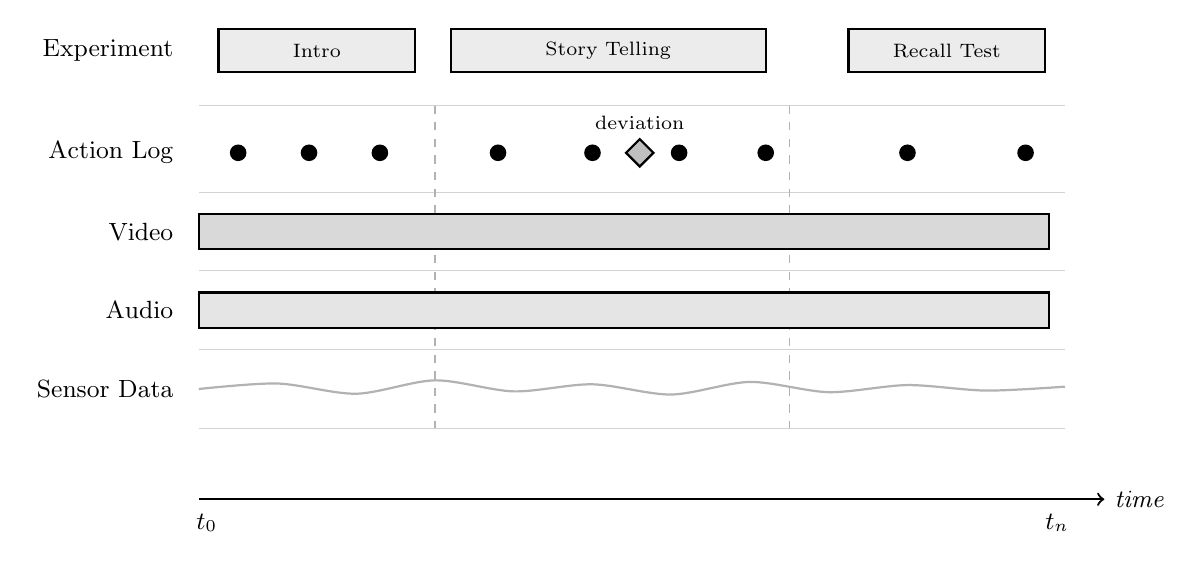
\begin{tikzpicture}[
    dot/.style={circle, fill=black, minimum size=6pt, inner sep=0pt},
    devdot/.style={rectangle, draw=black, thick, fill=gray!50, minimum size=7pt, inner sep=0pt, rotate=45},
    stepbox/.style={rectangle, draw=black, thick, fill=gray!15, align=center, font=\scriptsize, inner sep=3pt, minimum height=0.55cm},
    mediabar/.style={rectangle, draw=black, thick, fill=gray!30, minimum height=0.45cm},
    track/.style={font=\small, anchor=east}]

    % Time axis
    \draw[->, thick] (0, -0.5) -- (11.5, -0.5) node[right, font=\small\itshape] {time};
    \node[font=\small] at (0.1, -0.8) {$t_0$};
    \node[font=\small] at (10.9, -0.8) {$t_n$};

    % Track labels
    \node[track] at (-0.2, 5.2) {Experiment};
    \node[track] at (-0.2, 3.9) {Action Log};
    \node[track] at (-0.2, 2.9) {Video};
    \node[track] at (-0.2, 1.9) {Audio};
    \node[track] at (-0.2, 0.9) {Sensor Data};

    % Track dividers
    \foreach \y in {4.5, 3.4, 2.4, 1.4, 0.4} {
        \draw[gray!35, thin] (0, \y) -- (11.0, \y);
    }

    % Experiment step boxes
    \node[stepbox, minimum width=2.5cm] at (1.5, 5.2) {Intro};
    \node[stepbox, minimum width=4.0cm] at (5.2, 5.2) {Story Telling};
    \node[stepbox, minimum width=2.5cm] at (9.5, 5.2) {Recall Test};

    % Step boundary markers
    \draw[dashed, gray!60] (3.0, 4.5) -- (3.0, 0.4);
    \draw[dashed, gray!60] (7.5, 4.5) -- (7.5, 0.4);

    % Scripted actions
    \node[dot] at (0.5, 3.9) {};
    \node[dot] at (1.4, 3.9) {};
    \node[dot] at (2.3, 3.9) {};
    \node[dot] at (3.8, 3.9) {};
    \node[dot] at (5.0, 3.9) {};
    \node[dot] at (6.1, 3.9) {};
    \node[dot] at (7.2, 3.9) {};
    \node[dot] at (9.0, 3.9) {};
    \node[dot] at (10.5, 3.9) {};

    % Deviation marker
    \node[devdot] at (5.6, 3.9) {};
    \node[font=\scriptsize, above=5pt] at (5.6, 3.9) {deviation};

    % Video bar
    \node[mediabar, minimum width=10.8cm] at (5.4, 2.9) {};

    % Audio bar
    \node[mediabar, minimum width=10.8cm, fill=gray!20] at (5.4, 1.9) {};

    % Sensor data (continuous sampled line)
    \draw[thick, gray!60] plot[smooth] coordinates {
        (0.0, 0.90) (1.0, 0.97) (2.0, 0.84) (3.0, 1.01) (4.0, 0.87)
        (5.0, 0.96) (6.0, 0.83) (7.0, 0.99) (8.0, 0.86) (9.0, 0.95)
        (10.0, 0.88) (11.0, 0.93)
    };

\end{tikzpicture}
\caption{Structure of a completed trial record, showing synchronized action log, media, and sensor tracks.}
\label{fig:trial-record}
\end{figure}

Video and audio are recorded locally in the researcher's browser during the trial rather than streamed to the server in real time. This prevents network delays or server load from dropping frames or degrading audio quality during the interaction. When the trial concludes, the browser transfers the complete recordings to the server and associates them with the trial record. The Analysis interface can align video and audio with the logged actions without any manual synchronization, because the timestamp when recording starts is logged alongside the action log.

The system stores structured and media data separately. Experiment specifications and trial records live in a structured database, which makes it efficient to query across trials (for example, retrieving all trials for a specific participant or comparing action timing across conditions). Video and audio files live in a dedicated file store, since their size makes them unsuitable for a database and the system never queries their content directly.

\section{The Execution Engine}

The execution engine is the component that runs a live trial: it loads the experiment, manages the wizard's connection, dispatches robot commands, and keeps all connected clients in sync.

When a trial begins, the server loads the experiment and maintains a live connection to the wizard's browser and any observer connections. The execution engine does not advance the experiment on a timer; it waits for the wizard to trigger each step. This preserves the natural pacing of the interaction: the wizard advances only when the participant is ready, while the experiment structure ensures the protocol is followed. When the wizard triggers an action, the server dispatches the robot command, writes the log entry, and pushes the updated experiment state to all connected clients in the same operation — keeping the wizard's view, the observer view, and the actual robot state synchronized in real time.

No two participants respond identically. One subject gives a one-word answer; another offers a paragraph; a third asks the robot a question the script never anticipated. A fully programmed robot has no answer for that third subject: the interaction stalls, or immersion breaks. The wizard exists to fill that gap: where the program runs out of instructions, the wizard draws on their knowledge of human social interaction to keep the exchange coherent. Unscripted actions give the wizard the tools to exercise that judgment in the moment. The wizard triggers them via the manual controls in the Execution interface, the robot command runs, and the system logs the action with a deviation flag. This design preserves research value: the interaction gains the flexibility only a human can provide, and that flexibility appears explicitly in the record rather than disappearing into it.

\section{Robot Integration}

A configuration file describes each robot platform, listing the actions it supports and specifying how each one maps to a command the robot understands. The execution engine reads this file at startup and uses it whenever it needs to dispatch a command: it looks up the action type, assembles the appropriate message, and sends it to the robot over a bridge process running on the local network. The web server itself has no knowledge of any specific robot; all hardware-specific logic lives in the configuration file.

The execution engine treats control flow elements such as branches and conditionals the same way as robot actions. They appear as action groups in the experiment and resolve at runtime, so researchers can freely mix logical decisions and physical robot behaviors when designing an experiment without any special handling.

Figure~\ref{fig:plugin-architecture} illustrates this mapping using NAO6 and TurtleBot as an example. Actions a platform does not support (such as \texttt{raise\_arm} on TurtleBot) appear as explicitly unsupported in the configuration file rather than silently failing. The experiment itself does not change between platforms.

\begin{figure}[htbp]
\centering
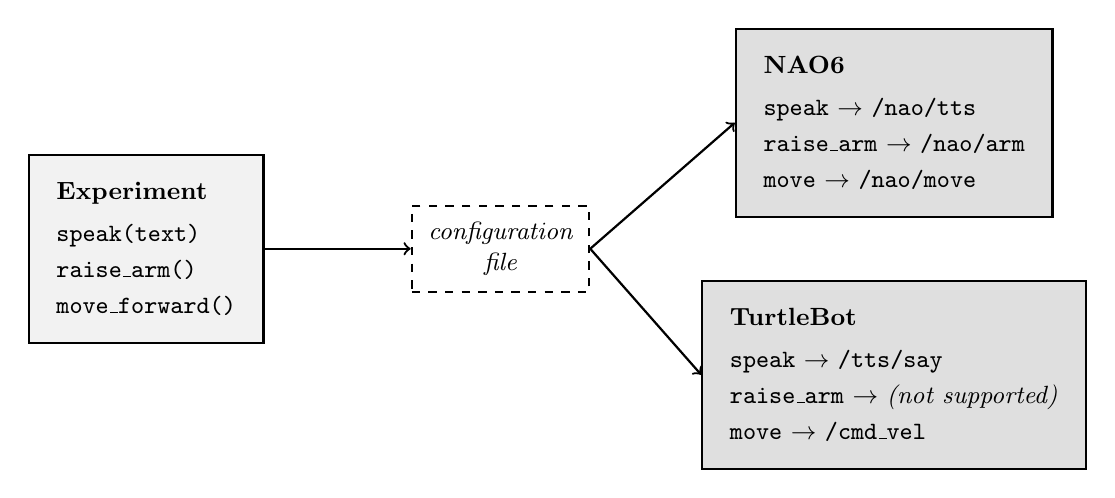
\begin{tikzpicture}[
    expbox/.style={rectangle, draw=black, thick, fill=gray!10, align=left, font=\small, inner sep=10pt},
    cfgbox/.style={rectangle, draw=black, thick, dashed, fill=white, align=center, font=\small\itshape, inner sep=6pt},
    robotbox/.style={rectangle, draw=black, thick, fill=gray!25, align=left, font=\small, inner sep=10pt},
    arrow/.style={->, thick}]

    % Experiment box
    \node[expbox] (exp) at (0, 0) {
        \textbf{Experiment}\\[4pt]
        \texttt{speak(text)}\\[2pt]
        \texttt{raise\_arm()}\\[2pt]
        \texttt{move\_forward()}
    };

    % Configuration file node (intermediate)
    \node[cfgbox] (cfg) at (4.5, 0) {configuration\\file};

    % NAO6 box
    \node[robotbox] (nao) at (9.5, 1.6) {
        \textbf{NAO6}\\[4pt]
        \texttt{speak} $\to$ \texttt{/nao/tts}\\[2pt]
        \texttt{raise\_arm} $\to$ \texttt{/nao/arm}\\[2pt]
        \texttt{move} $\to$ \texttt{/nao/move}
    };

    % TurtleBot box
    \node[robotbox] (tb) at (9.5, -1.6) {
        \textbf{TurtleBot}\\[4pt]
        \texttt{speak} $\to$ \texttt{/tts/say}\\[2pt]
        \texttt{raise\_arm} $\to$ \textit{(not supported)}\\[2pt]
        \texttt{move} $\to$ \texttt{/cmd\_vel}
    };

    % Arrows
    \draw[arrow] (exp.east) -- (cfg.west);
    \draw[arrow] (cfg.east) -- (nao.west);
    \draw[arrow] (cfg.east) -- (tb.west);

\end{tikzpicture}
\caption{Abstract experiment actions translated to platform-specific robot commands through per-platform configuration files.}
\label{fig:plugin-architecture}
\end{figure}

\section{Access Control}

I implemented access control using a role-based access control (RBAC) model. Each study has a membership list, and every member is assigned one of four roles that define a clear separation of duties: those who own the study, those who design it, those who run it, and those who observe it. This enforces need-to-know access at the study level so that each team member sees only what their role requires.

\begin{description}
    \item[Owner.] Full control over the study: can invite or remove members, configure the study settings, and access all data.
    \item[Researcher.] Can create and modify experiment designs and review all collected trial data, but cannot manage team membership.
    \item[Wizard.] Can trigger actions during a live trial and view the execution interface, but cannot modify the experiment design or access other wizards' sessions.
    \item[Observer.] Read-only access: can watch a live trial in real time and annotate significant moments, but cannot trigger actions or modify any data.
\end{description}

The role system also supports double-blind designs~\cite{Bartneck2024}: the Owner can restrict a Wizard's view of condition assignments, and restrict Researchers from accessing result data until the study concludes, without any changes to the underlying experiment.

\section{Architectural Challenges}

Two problems required specific solutions during implementation.

\begin{description}
    \item[Execution latency.] During a live trial, the execution engine must respond quickly to wizard input — a noticeable delay between the button press and the robot's action can disrupt the interaction. I addressed this by maintaining a persistent connection for the duration of each trial. The connection is established once at trial start and kept open, eliminating per-action setup overhead.

    \item[Multi-source synchronization.] Analysis requires aligning data streams captured at different sampling rates by different components: video, audio, action logs, and sensor data. The solution is a shared time reference: every data source records its timestamps relative to the same trial start time, $t_0$, so the Analysis interface can align all tracks without requiring manual calibration. This is the timestamp structure shown in Figure~\ref{fig:trial-record}.
\end{description}

\section{Implementation Status}

HRIStudio has reached minimum viable product status. The Design, Execution, and Analysis interfaces are operational. The execution engine handles scripted and unscripted actions with full timestamped logging, and I validated robot communication on the NAO6 platform during development. The platform can run a controlled WoZ study without modification.

Work remaining for future development includes support for studies that use more than one robot at a time and validation of the configuration file approach on robot platforms beyond NAO6.

\section{Chapter Summary}

This chapter described how HRIStudio realizes the design concepts from Chapter~\ref{ch:design} in practice. Experiments are persistent, reusable specifications that produce complete, comparable trial records. The execution engine is event-driven rather than timer-driven, keeping the wizard in control of pacing while logging every action automatically. Per-platform configuration files keep the execution engine hardware-agnostic. The role system enforces access control at the study level. The platform is at minimum viable product status and can run a controlled WoZ study today. HRIStudio is one realization of these concepts; the contribution lies in the design principles themselves, which any implementation could adopt.

\chapter{Pilot Validation Study}
\label{ch:evaluation}

This chapter presents the pilot validation study used to evaluate whether HRIStudio improves accessibility and reproducibility in WoZ-based HRI research. It defines the research questions, study design, task, apparatus, procedure, and measurement instruments.

\section{Research Questions}

The validation study targets the two problems established in Chapter~\ref{ch:background}. The first is the \emph{Accessibility Problem}: existing tools require substantial programming expertise, which prevents domain experts from conducting independent HRI studies. The second is the \emph{Reproducibility Problem}: without structured logging and protocol enforcement, experiment execution varies across participants and wizards in ways that are difficult to detect or control after the fact.

These problems give rise to two research questions. The first is whether HRIStudio enables domain experts without prior robotics experience to successfully implement a robot interaction from a written specification. The second is whether HRIStudio produces more reliable execution of that interaction compared to standard practice.

I hypothesized that HRIStudio would improve both accessibility and reproducibility compared to Choregraphe: wizards using HRIStudio would more completely and correctly implement the written specification, and their designs would execute more reliably during the trial.

\section{Study Design}

I used what Bartneck et al.~\cite{Bartneck2024} call a \emph{between-subjects design}, in which each participant is assigned to only one condition. To ensure that programming experience was balanced across conditions, I stratified assignment by self-reported programming background: each wizard was first classified as having \emph{None}, \emph{Moderate}, or \emph{Extensive} programming experience, and then randomly assigned within that stratum to HRIStudio or Choregraphe. This produced a design in which each condition contained exactly one wizard at each experience level, reducing the risk that tool effects would be confused with differences in programming experience. Both groups received the same task, the same time allocation, and a similar training structure. Because each wizard used only one tool, the design also avoided carryover effects from prior exposure to the other condition.

\section{Participants}

\textbf{Wizards.} A primary claim of HRIStudio is that it lowers the technical barrier for domain experts who are not programmers; testing this claim with its intended user population was therefore a primary goal of participant recruitment. I recruited six Bucknell University faculty members drawn from across departments to serve as wizards, deliberately targeting both ends of the programming experience spectrum: those with substantial programming backgrounds as well as those who described themselves as non-programmers or having minimal coding experience. Drawing wizards from outside computer science allows the data to speak to whether that claim holds for the intended user population.

The key inclusion criterion for all wizards was no prior experience with either the NAO robot or Choregraphe software specifically. This controls for tool familiarity so that performance differences reflect the tools themselves rather than prior exposure. I recruited wizards through direct email, and participation was framed as a voluntary software evaluation unrelated to any professional obligations.

\textbf{Sample size rationale.} I chose to recruit six wizard participants ($N = 6$), believing that this sample size is appropriate for a pilot validation study whose goal is directional evidence and failure-mode identification rather than effect-size estimation for a broad population. This scale is consistent with pilot and feasibility studies in HRI, where small $N$ designs are common in early-stage tool validation~\cite{HoffmanZhao2021}. Findings should be interpreted as preliminary evidence and directional indicators rather than as conclusive substantiation of any claims.

\section{Task}

The task chosen was to have a robot tell a story to a human subject and later evaluate if that subject could recall a specific detail.

Both wizard groups received the same written task specification: the \emph{Interactive Storyteller} scenario. The specification described a robot that introduces an astronaut named Kai, narrates her discovery of a red rock on Mars, asks a recall question, and delivers a response according to the answer given. The full specification, including exact robot speech, required gestures, and branching logic, is reproduced in Appendix~\ref{app:blank_templates}. This scenario is representative of HRI tasks in which a robot conveys information to a human subject; one might, for example, measure whether a robot or human storyteller produces better recall in subjects.

This scenario was chosen because it requires several distinct capabilities: speech actions, gesture coordination, conditional branching, and a defined conclusion. In both conditions, wizards had to translate the same written protocol into an executable interaction script, including action ordering, branching logic, and timing decisions. In Choregraphe, that meant assembling and connecting behavior nodes in a finite state machine. In HRIStudio, it meant building a sequential action timeline with conditional branches. This makes the task a direct comparison of how each tool supports coding the robot behavior required by the same protocol.

\section{Robot Platform and Software Apparatus}

Both conditions used the same NAO humanoid robot (Figure~\ref{fig:nao6-photo}), a platform approximately 0.58 meters tall capable of speech synthesis, animated gestures, and head movement. Using the same hardware ensured that any differences in execution quality were attributable to the software, not the robot.


\begin{figure}[htbp]
\centering
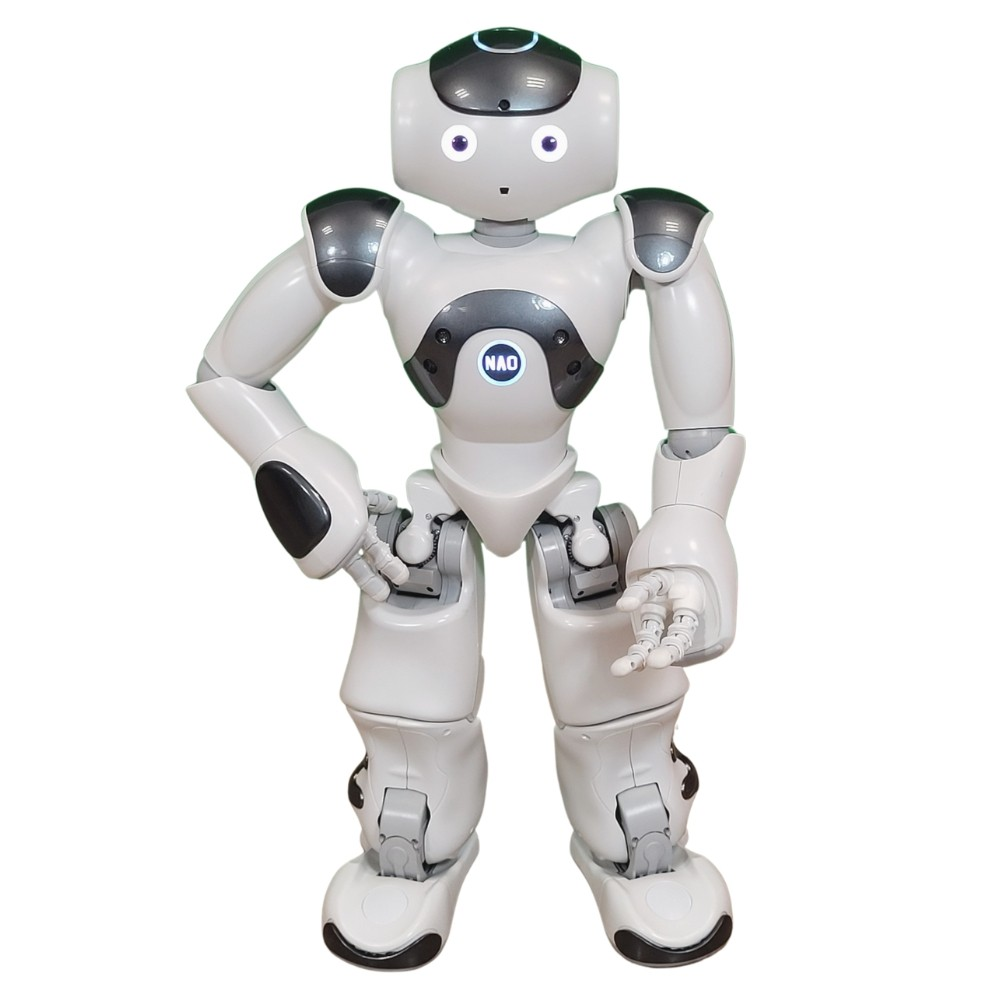
\includegraphics[width=0.45\textwidth]{images/nao6.jpg}
\caption{The NAO6 humanoid robot used in both conditions of the pilot study.}
\label{fig:nao6-photo}
\end{figure}


The control condition used Choregraphe \cite{Pot2009}, a proprietary visual programming tool developed by Aldebaran Robotics and the standard software for NAO programming. Choregraphe organizes behavior as a finite state machine: nodes represent states and edges represent transitions triggered by conditions or timers.

The experimental condition used HRIStudio, described in Chapter~\ref{ch:implementation}. HRIStudio organizes behavior as a sequential action timeline with support for conditional branches. Unlike Choregraphe, it abstracts robot-specific commands through plugin files, though for this study both tools controlled the same NAO platform.

Figure~\ref{fig:design-tool-compare} places the two design environments side by side. On the left, Choregraphe's behavior-box canvas (Figure~\ref{fig:choregraphe-ui}) lets the wizard wire nodes and transitions in a finite-state-machine layout. On the right, HRIStudio's experiment designer (Figure~\ref{fig:hristudio-designer}) presents the same protocol as a vertical action timeline with dedicated blocks for speech, gesture, and conditional branching.

\begin{figure}[htbp]
\centering
\begin{minipage}[t]{0.48\textwidth}
\centering
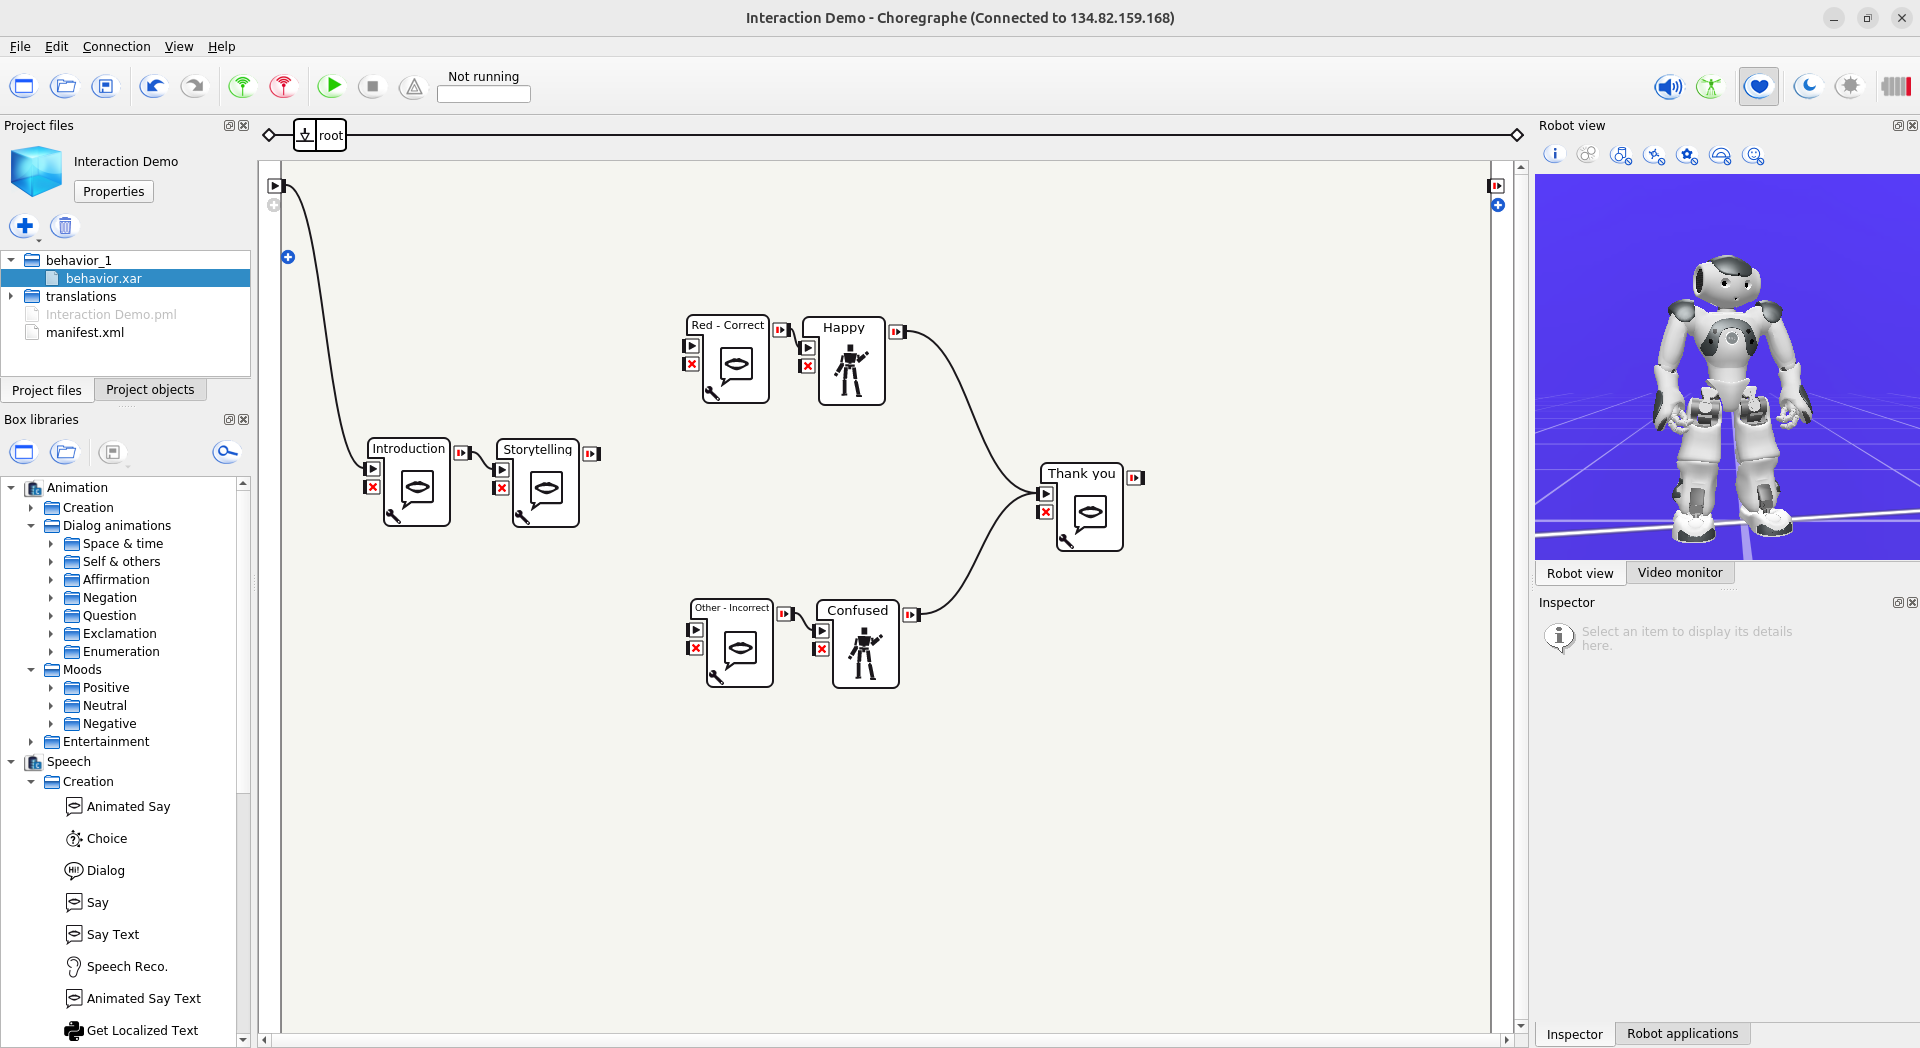
\includegraphics[width=\textwidth]{assets/choregraphe.png}
\subcaption{Choregraphe: behavior-box canvas with nodes and transitions.}
\label{fig:choregraphe-ui}
\end{minipage}\hfill
\begin{minipage}[t]{0.48\textwidth}
\centering
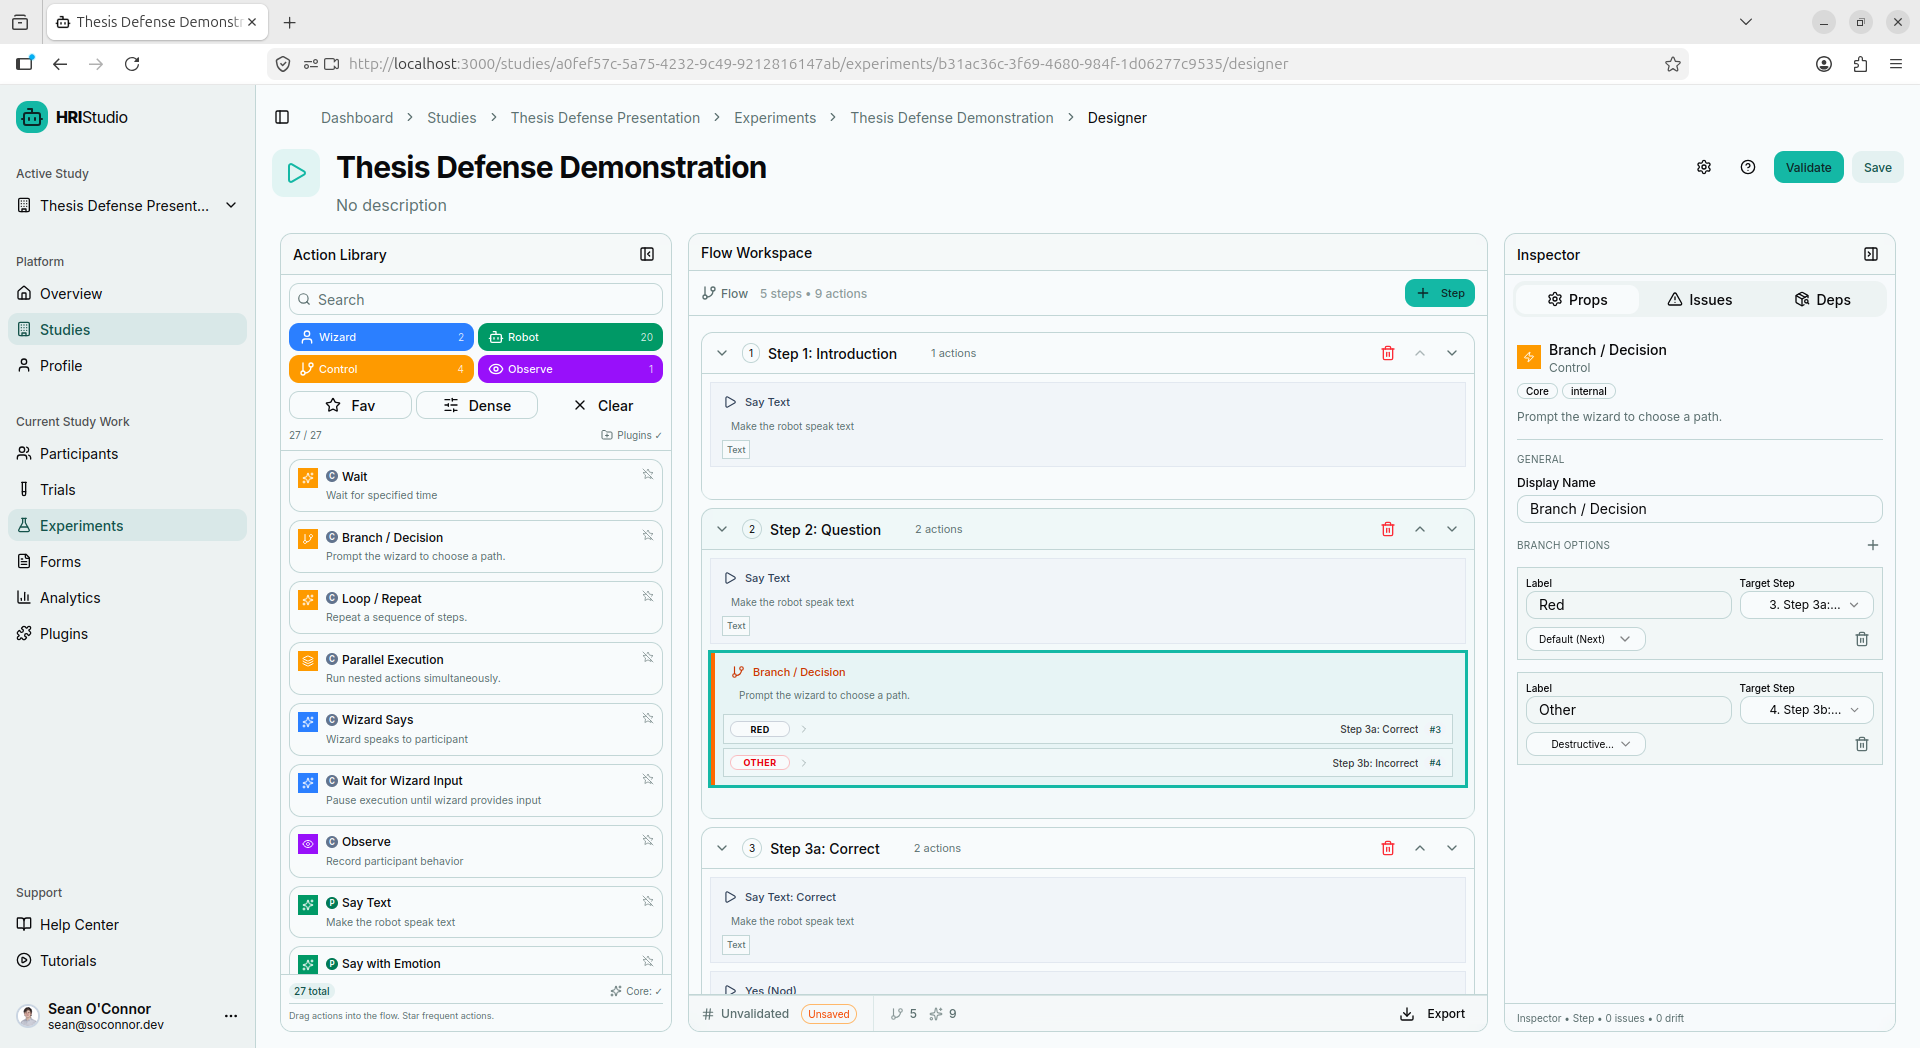
\includegraphics[width=\textwidth]{assets/experiment-designer.png}
\subcaption{HRIStudio: vertical action timeline with structured step and action blocks.}
\label{fig:hristudio-designer}
\end{minipage}
\caption{The two design environments compared. Each wizard used one of these tools to implement the Interactive Storyteller specification.}
\label{fig:design-tool-compare}
\end{figure}

\section{Procedure}

Each wizard completed a single 60-minute session structured in four phases.

\subsection{Phase 1: Training (15 minutes)}

I opened each session with a standardized tutorial tailored to the wizard's assigned tool. The tutorial covered how to create speech actions, specify gestures, define conditional branches, and save the completed design. Training was intentionally allocated 15 minutes to allow enough time for wizards to ask clarifying questions about the tool before the design challenge began, while still simulating first encounter with a new tool without extensive onboarding. I answered clarification questions during this phase but did not offer hints about the design challenge.

\subsection{Phase 2: Design Challenge (30 minutes)}

The wizard received the specification and had 30 minutes to implement it using their assigned tool. Using a structured observer data sheet (found in Appendix~\ref{app:blank_templates}), I logged every instance in which I provided assistance to the wizard, categorizing each by type: \emph{tool-operation} (T), \emph{task clarification} (C), \emph{hardware or technical} (H), or \emph{general} (G). For each tool-operation intervention, I also recorded which rubric item it pertained to. If the wizard declared completion before the time limit, the remaining time was used to review and refine the design.

\subsection{Phase 3: Live Trial (10 minutes)}

After the design phase, the wizard ran their completed program to execute the designed interaction on the robot. I continued logging any researcher interventions during the trial using the same type categories, noting the relevant ERS rubric item for any tool-operation intervention.

\subsection{Phase 4: Debrief (5 minutes)}

Following the trial, the wizard completed the System Usability Scale survey (found in Appendix~\ref{app:blank_templates}). The DFS and ERS were scored during and immediately after the session using live observation and the Observer Data Sheet.

\section{Measures}
\label{sec:measures}

The study collected five measures, two primary and three supplementary, operationalized through five instruments. They are described as follows.

\subsection{Design Fidelity Score}

I define the Design Fidelity Score (DFS) as a measure of how completely and correctly the wizard implemented the specification. I evaluated the exported project file against nine weighted criteria grouped into three categories: speech actions, gestures and actions, and control flow and logic. Each criterion is scored as present, correct, and independently achieved.

The DFS rubric includes an \emph{Assisted} column. For each rubric item, I marked a T if I provided a tool-operation intervention specifically for that item during the design phase (for example, if I explained how to add a gesture node or how to wire a conditional branch). T marks are recorded and reported separately alongside the DFS score; they do not affect the Points total. This preserves the DFS as a clean measure of design fidelity while providing a parallel record of where tool-specific assistance was needed. General interventions (task clarification, hardware issues, or momentary forgetfulness) are not marked T, because those categories of difficulty are independent of the tool under evaluation.

DFS is motivated by a gap identified by Riek~\cite{Riek2012}, whose systematic review of 54 published WoZ studies found that only 11\% constrained wizard behavior and fewer than 6\% described wizard training procedures. Porfirio et al.~\cite{Porfirio2023} similarly argued that formal, verifiable behavior specifications are a prerequisite for reproducible HRI. The DFS applies these recommendations as a weighted rubric scored against the exported project file. The complete rubric is reproduced in Appendix~\ref{app:blank_templates}. This measure addresses the question: did the tool allow a wizard to independently produce a correct design?

\subsection{Execution Reliability Score}

I define the Execution Reliability Score (ERS) as a measure of whether the designed interaction executed as intended during the live trial. I scored the ERS live and immediately after the session, using the Observer Data Sheet and the wizard's exported project file. Evaluation criteria included whether the robot delivered the correct speech at each step, whether gestures executed and synchronized with speech, whether the conditional branch was present in the design and executed during the trial, and whether any errors, disconnections, or hangs occurred.

The ERS rubric applies the same \emph{Assisted} modifier as the DFS, extended to the trial phase. Any tool-operation intervention I provided during the trial (for example, explaining to the wizard how to launch or advance their program) caps the affected ERS item at half points. This is scored separately from design-phase interventions: a wizard who needed help only during design can still achieve a full ERS score if the trial runs without assistance, and vice versa. The rubric records whether the trial reached its conclusion step. I additionally note whether any branch resolved through programmed conditional logic or through manual intervention by the wizard during execution.

This measure responds directly to Riek's~\cite{Riek2012} finding that only 3.7\% of published WoZ studies reported any measure of wizard error, making it nearly impossible to determine whether execution matched design intent~\cite{OConnor2024, OConnor2025}. The complete rubric is reproduced in Appendix~\ref{app:blank_templates}. This measure addresses the question: did the design translate reliably into execution without researcher support?

\subsection{System Usability Scale}

The System Usability Scale (SUS) is a validated 10-item questionnaire measuring perceived usability, created by Brooke~\cite{Brooke1996}. Wizards completed the SUS after the debrief phase. Scores range from 0 to 100, with higher scores indicating better perceived usability. The full questionnaire is reproduced in Appendix~\ref{app:blank_templates}.

\subsection{Intervention Log and Session Timing}

During each session, I maintained a structured intervention log on the observer data sheet, recording the timestamp, type code, affected rubric item number, and a brief description for every instance in which I assisted the wizard. The four intervention type codes are:

\begin{description}
    \item[T (tool-operation).] I explained how to operate a specific feature of the assigned software tool.
    \item[C (task clarification).] I clarified the written specification or an aspect of the task design.
    \item[H (hardware or technical).] I addressed a robot connection issue or other technical problem outside the wizard's control.
    \item[G (general).] Brief assistance not attributable to the tool or the task, such as momentary forgetfulness.
\end{description}

Only T-type interventions affect rubric scoring; the others are recorded to provide context for interpreting session flow and wizard experience. I also recorded the actual duration of each session phase and the time at which the wizard completed or abandoned the design, providing supplementary evidence about tool accessibility beyond the DFS score itself.

\section{Measurement Instruments}

The five measures are designed to work together. The DFS and ERS address separate phases of the session: DFS captures what was designed, and ERS captures whether that design translated faithfully into execution. Taken together, they make it possible to distinguish a wizard who implemented the specification correctly but whose design failed during the trial from one whose design was incomplete but executed without researcher assistance. The SUS grounds both scores in the wizard's subjective experience of the tool. The intervention log and session timing are supplementary: they do not directly answer the research questions but provide context for interpreting the primary scores, particularly for understanding whether help requests concerned the tool itself or the task.

Table~\ref{tbl:measurement_instruments} summarizes the five instruments, when they were collected, and which research question each addresses.

\begin{table}[htbp]
\centering
\footnotesize
\begin{tabular}{|p{3.0cm}|p{4.4cm}|p{2.4cm}|p{2.8cm}|}
\hline
\textbf{Instrument} & \textbf{What it captures} & \textbf{When collected} & \textbf{Research question} \\
\hline
Design Fidelity Score (DFS) & Completeness and correctness of the wizard's implementation; caps items where tool-operation assistance was given & Post-session file review & Accessibility \\
\hline
Execution Reliability Score (ERS) & Whether the interaction executed as designed during the trial; caps items where trial-phase tool assistance occurred & Live and post-trial (ODS) & Reproducibility \\
\hline
System Usability Scale (SUS) & Wizard's perceived usability of the assigned tool & Debrief phase & User experience \\
\hline
Intervention Log & Timestamped record of all researcher assistance by type (T/C/H/G) and affected rubric item & Throughout session & Supplementary \\
\hline
Session Timing & Actual duration of each phase; time to design completion & Throughout session & Supplementary \\
\hline
\end{tabular}
\caption{Measurement instruments used in the pilot validation study.}
\label{tbl:measurement_instruments}
\end{table}

\section{Chapter Summary}

This chapter described the structure of a pilot between-subjects study I designed to test whether the design principles formalized in Chapters~\ref{ch:design} and~\ref{ch:implementation} produce measurably different outcomes from existing practice. Six wizard participants ($N = 6$), drawn from across departments and spanning the programming experience spectrum, each designed and ran the Interactive Storyteller task on a NAO robot using either HRIStudio or Choregraphe. Each 60-minute session was structured in four phases: a 15-minute standardized tutorial, a 30-minute design challenge, a 10-minute live trial, and a 5-minute debrief. I measured design fidelity (DFS) and execution reliability (ERS) against the written specification, applying a per-item scoring modifier that caps any rubric criterion for which tool-operation assistance was given. I also collected perceived usability via the SUS, a structured intervention log categorizing all researcher assistance by type, and session phase timings. Chapter~\ref{ch:results} presents the results.

\chapter{Results}
\label{ch:results}

\section{Quantitative Results}
% TODO

\section{Qualitative Findings}
% TODO

\chapter{Discussion}
\label{ch:discussion}

\section{Interpretation of Findings}
% TODO

\section{Comparison to Prior Work}
% TODO

\section{Limitations}
% TODO

\chapter{Conclusion and Future Work}
\label{ch:conclusion}

This thesis set out to address two persistent problems in Wizard-of-Oz-based social robotics research. The first is the Accessibility Problem: a high technical barrier prevents domain experts who are not programmers from conducting HRI studies independently. The second is the Reproducibility Problem: the fragmented landscape of custom tools makes it difficult to verify or replicate experimental results across studies and labs. This chapter summarizes the contributions of the work, reflects on what the pilot study results suggest, and identifies directions for future investigation.

\section{Contributions}

This thesis makes three contributions to the field of HRI research infrastructure.

\textbf{A principled architecture for WoZ platforms.} The primary contribution is a set of design principles for Wizard-of-Oz infrastructure: a hierarchical specification model (Study $\to$ Experiment $\to$ Step $\to$ Action), an event-driven execution model that separates protocol design from live trial control, and a plugin architecture that decouples experiment logic from robot-specific implementations. These principles are not specific to any one robot platform or research group; they describe a general approach to building WoZ tools that are simultaneously accessible to non-programmers and reproducible across executions. The principles were derived from a systematic analysis of reproducibility failures in published WoZ literature, grounded in the prior work of Riek~\cite{Riek2012} and Porfirio et al.~\cite{Porfirio2023}, and refined through the design and implementation process described in Chapters~\ref{ch:design} and~\ref{ch:implementation}.

\textbf{HRIStudio: a complete, operational platform.} The second contribution is HRIStudio, an open-source, web-based platform that fully realizes the design principles described above. HRIStudio is distributed under the MIT License and available at a public repository. HRIStudio provides a visual experiment designer, a consolidated wizard execution interface, role-based access control for research teams, and a repository-based plugin system for integrating robot platforms including the NAO6 used in this study. HRIStudio demonstrates that the design principles are not only technically feasible but can be delivered as a complete system that real researchers use without programming expertise, making it both an artifact and an instrument of validation. The platform's architecture is documented in detail in Chapter~\ref{ch:implementation} and the accompanying technical appendix.

\textbf{Pilot empirical evidence.} The third contribution is a pilot between-subjects study comparing HRIStudio against Choregraphe as a representative baseline tool. While the pilot scale precludes inferential claims, the study provides directional evidence on both research questions and produces a concrete demonstration of the reproducibility problem in a controlled setting: a wizard using Choregraphe deviated from the written specification in a way that was undetected until the live trial. This incident motivates the enforcement model at the core of HRIStudio's design and illustrates why the reproducibility problem is difficult to solve through training or norms alone.

\section{Reflection on Research Questions}

The central question this thesis addressed was: \emph{can the right software architecture make Wizard-of-Oz experiments more accessible to non-programmers and more reproducible across participants?} The evidence from the pilot study suggests the answer is yes, with the qualifications appropriate to a small $N$ directional study.

On accessibility, all three HRIStudio sessions produced a perfect DFS of 100, with design phases averaging 21 minutes, all within the allocation. The most direct demonstration comes from W-05: a Chemical Engineering faculty member with no programming background trained in 6 minutes, completed a perfect design in 18 minutes, and ran the trial to conclusion. SUS scores reflect the same directional split: Choregraphe mean 59.2 (below the average benchmark of 68), HRIStudio mean 76.7 (above it).

On reproducibility, the content deviation observed in W-01's Choregraphe session (see Section~\ref{sec:results-qualitative}) illustrates the failure mode the reproducibility problem predicts. No equivalent deviation occurred in any HRIStudio session. Branching was present and executed correctly in all three HRIStudio trials; ERS means reflect the outcome: 66.7 for Choregraphe, 96.7 for HRIStudio.

\section{Future Directions}

The work described in this thesis suggests several directions for future investigation.

\textbf{Larger validation study.} The most immediate next step is a full-scale study with sufficient participants to support inferential analysis. A sample of 20 or more wizard participants, balanced across programming backgrounds and conditions, would allow the DFS and ERS comparisons to be evaluated for statistical significance. A larger study would also enable subgroup analysis, for example whether the accessibility benefit of HRIStudio is concentrated among non-programmers or extends equally to programmers.

\textbf{Evaluations with multiple different tasks.} The Interactive Storyteller is a simple single-interaction task with one conditional branch. Real HRI experiments are more complex: they involve multiple conditions, longer interactions, and more elaborate branching logic. Evaluating HRIStudio on richer specifications would test whether the accessibility and reproducibility benefits scale with task complexity, and whether any new limitations emerge at that scale.

\textbf{Longitudinal use.} This study evaluated first-session performance, which captures the initial learning curve but not longer-term practice. A longitudinal study tracking wizard performance across multiple sessions would reveal whether HRIStudio's benefits persist or diminish as wizards become proficient, and whether the tool's structured approach continues to enforce reproducibility over time.

\textbf{Observer and researcher roles.} HRIStudio's role-based architecture includes Observer and Researcher roles that were not formally evaluated in this study. Future work should investigate how these roles support team coordination in multi-experimenter studies, and whether the annotation and logging capabilities they enable produce analysis workflows that are meaningfully more efficient than manual video coding.

\textbf{Platform expansion.} The NAO integration used in this study is one instance of HRIStudio's plugin architecture. Extending the plugin ecosystem to include mobile robots, socially assistive robots, and non-humanoid platforms would broaden the system's applicability and test whether the plugin abstraction is sufficiently general to accommodate the range of robot capabilities used in published HRI research.

\textbf{Community adoption.} The reproducibility problem in WoZ research is ultimately a community problem, not a tool problem. Future work should investigate what it would take for HRIStudio to be adopted as shared infrastructure across multiple labs, including documentation standards, experiment sharing mechanisms, and incentive structures that make reproducibility a norm rather than an exception.

\section{Closing Remarks}

The Wizard-of-Oz technique is one of the most powerful tools available to HRI researchers: it allows the study of interaction designs that do not yet exist as autonomous systems, accelerating the feedback loop between design intuition and empirical evidence. But the technique has been practiced for decades without the infrastructure needed to make it systematic. Studies are conducted with custom tools that are not always shared, by wizards whose behavior is never verified against a protocol, producing results that cannot be replicated because the exact conditions that produced them were never precisely recorded.

HRIStudio is an attempt to build that infrastructure. It will not solve the reproducibility problem by itself; that requires community norms, institutional incentives, and continued investment in open, shared tooling. But it demonstrates that the technical barriers are not insurmountable: a web-based platform can make WoZ research accessible to domain experts who are not engineers, and execution enforcement can prevent the kinds of specification drift that silently degrade research quality. That is, at minimum, where the work begins.


\backmatter
%\bibliographystyle{thesis_num}   %This uses BU thesis file thesis_num.bst
%\bibliographystyle{abbrvnat}
\bibliographystyle{unsrtnat}
%\bibliographystyle{plainnat}

%%%%Use following line if bibtex is being used.
\bibliography{refs.bib}


%%%Use following if references are being entered by hand.
%\begin{thebibliography}{99}
%\bibitem[Smith(2005)]{SMI05}J.~Smith, ``An even better paper,''
%J.~Better Phys., {\bf 2}, 294 (2005).
%\bibitem[Ligare(2004)]{LIG04}M.~Ligare, ``A very good paper,''
%J.~Good Phys., {\bf 2}, 294 (2004).
%\end{thebibliography}

\makeatletter\@mainmattertrue\makeatother
\appendix
\chapter{Blank Study Templates}
\label{app:blank_templates}

This appendix contains the blank versions of all study instruments used in the pilot validation study. These templates were used to produce the completed materials in Appendix~\ref{app:completed_materials}.

A note on the Informed Consent Form (ICF): the ICF was submitted with the original protocol to the Bucknell University Institutional Review Board (Protocol \#2526-025) and reflects the study design as initially proposed. The protocol was refined before data collection began; the key differences between the ICF and the executed protocol are as follows. First, phase durations were adjusted: Training was planned at 15 minutes, the Design Challenge at 30 minutes, the Live Trial at 10 minutes, and the Debrief at 5 minutes, rather than the 10/20/15/15-minute allocations stated in the ICF. Second, screen recording during the design phase was not implemented, as the DFS is scored from the exported project file rather than from screen footage. Third, the live trial was conducted with the researcher serving as the test subject rather than a recruited student volunteer, as discussed in Chapter~\ref{ch:evaluation}. The ODS, DFS, ERS, and SUS templates reflect the protocol as executed.

\medskip
\noindent\textbf{Contents of this appendix, in order:} ODS, DFS, ERS, SUS, ICF

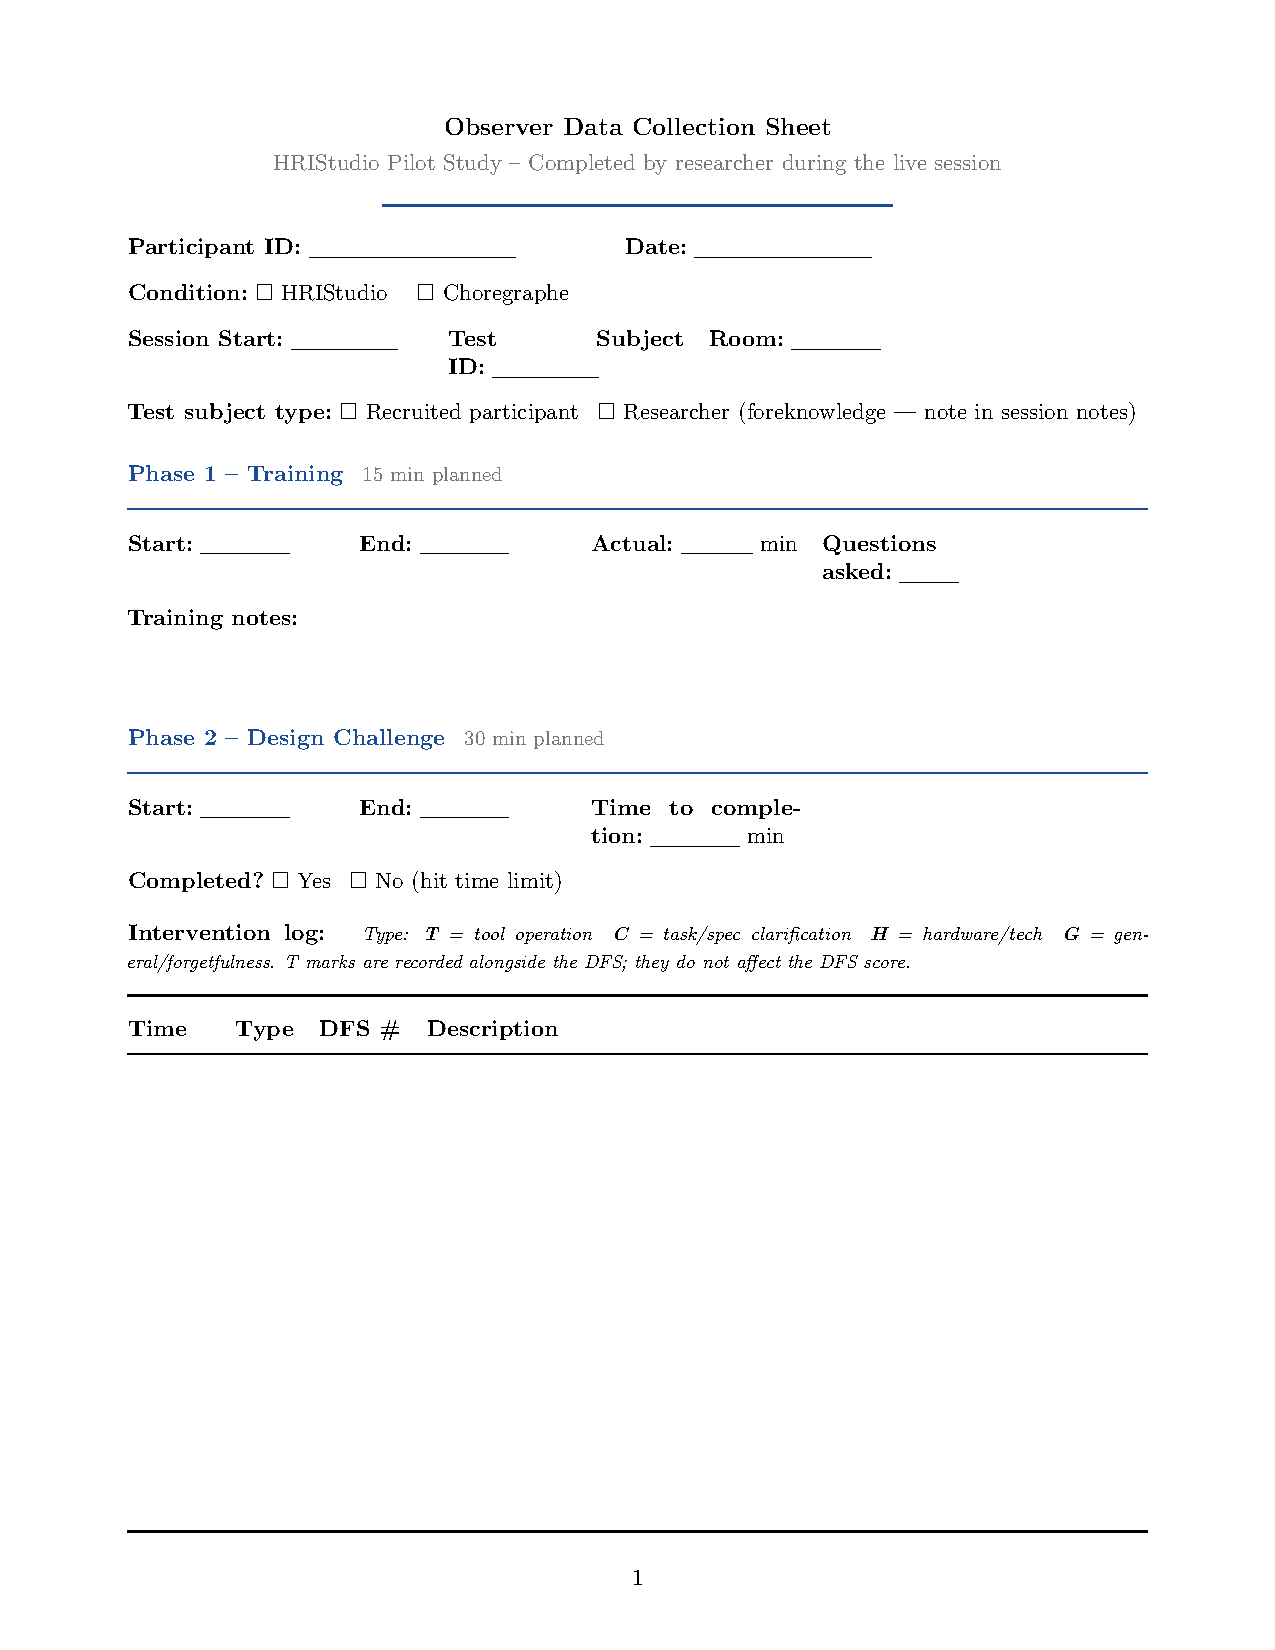
\includepdf[pages=-,pagecommand={}]{pdfs/templates/ODS-Template.pdf}
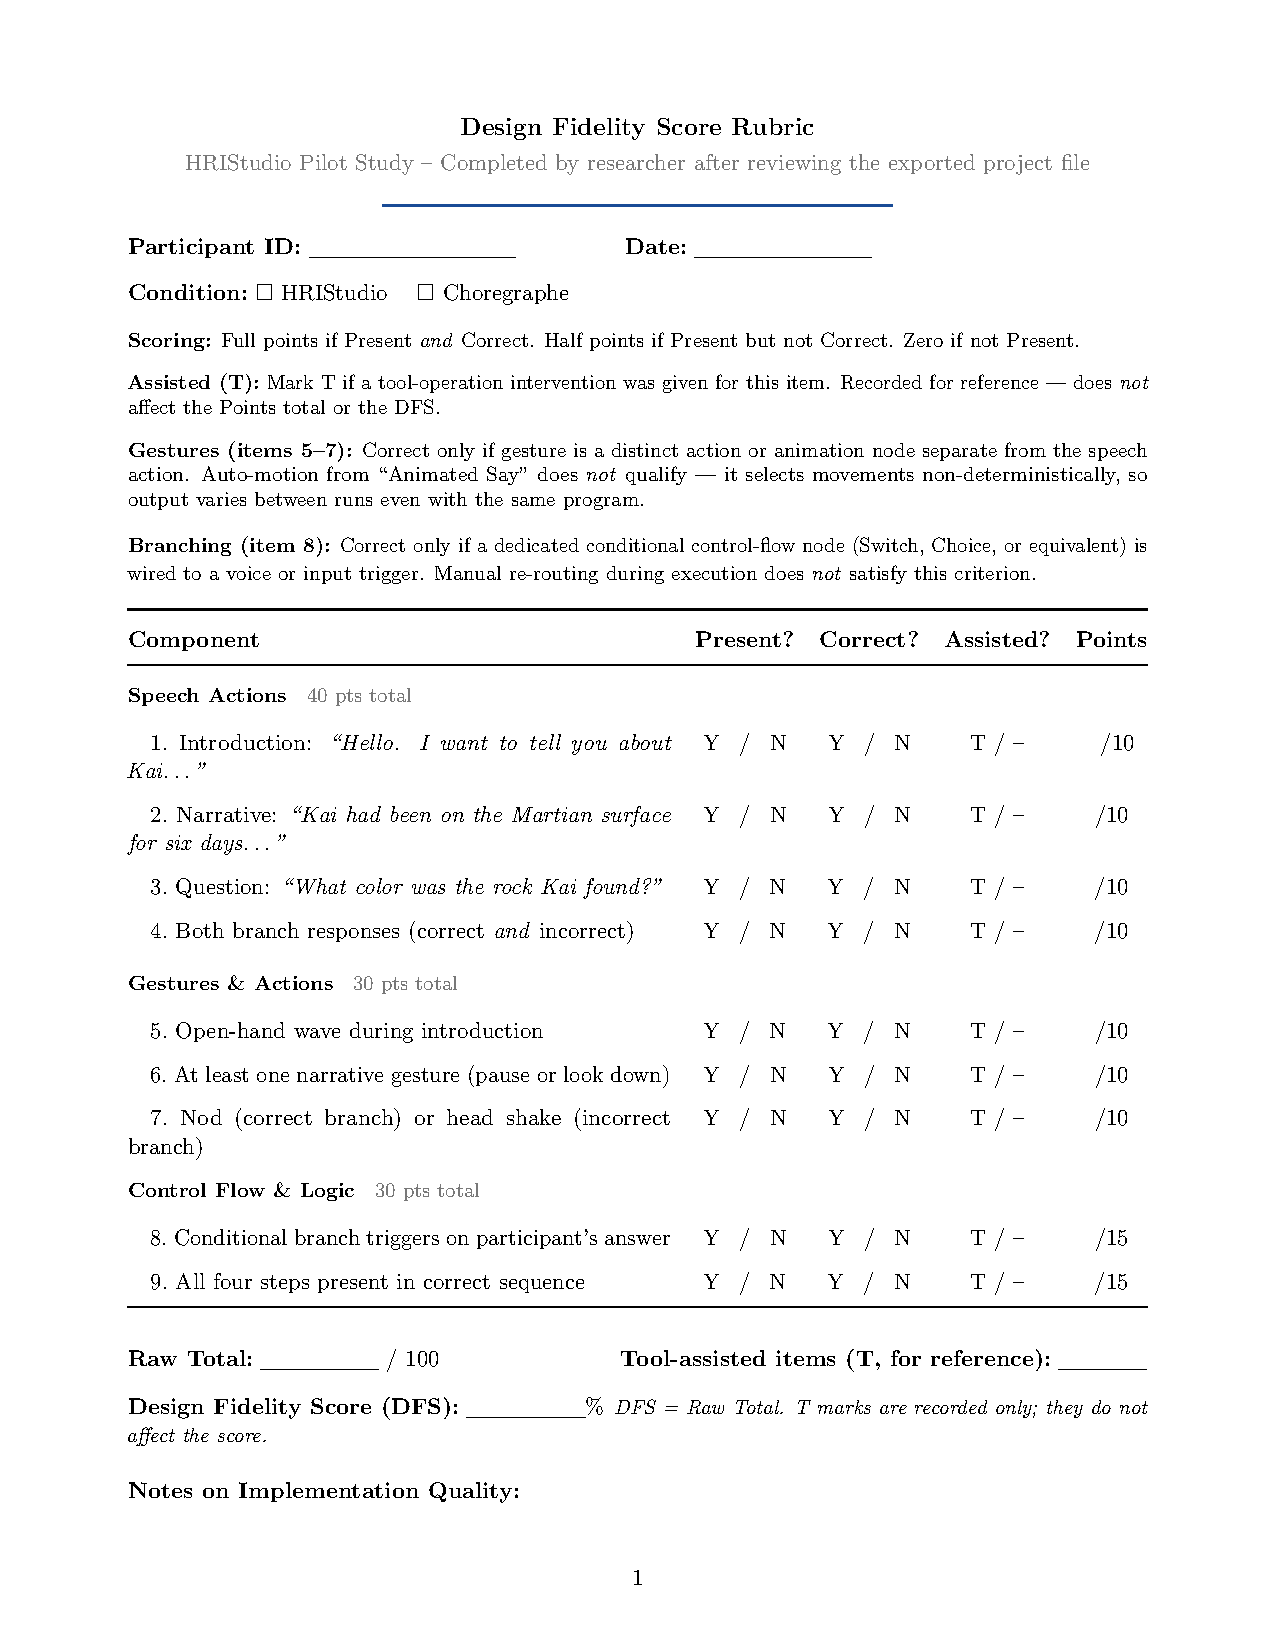
\includepdf[pages=-,pagecommand={}]{pdfs/templates/DFS-Template.pdf}
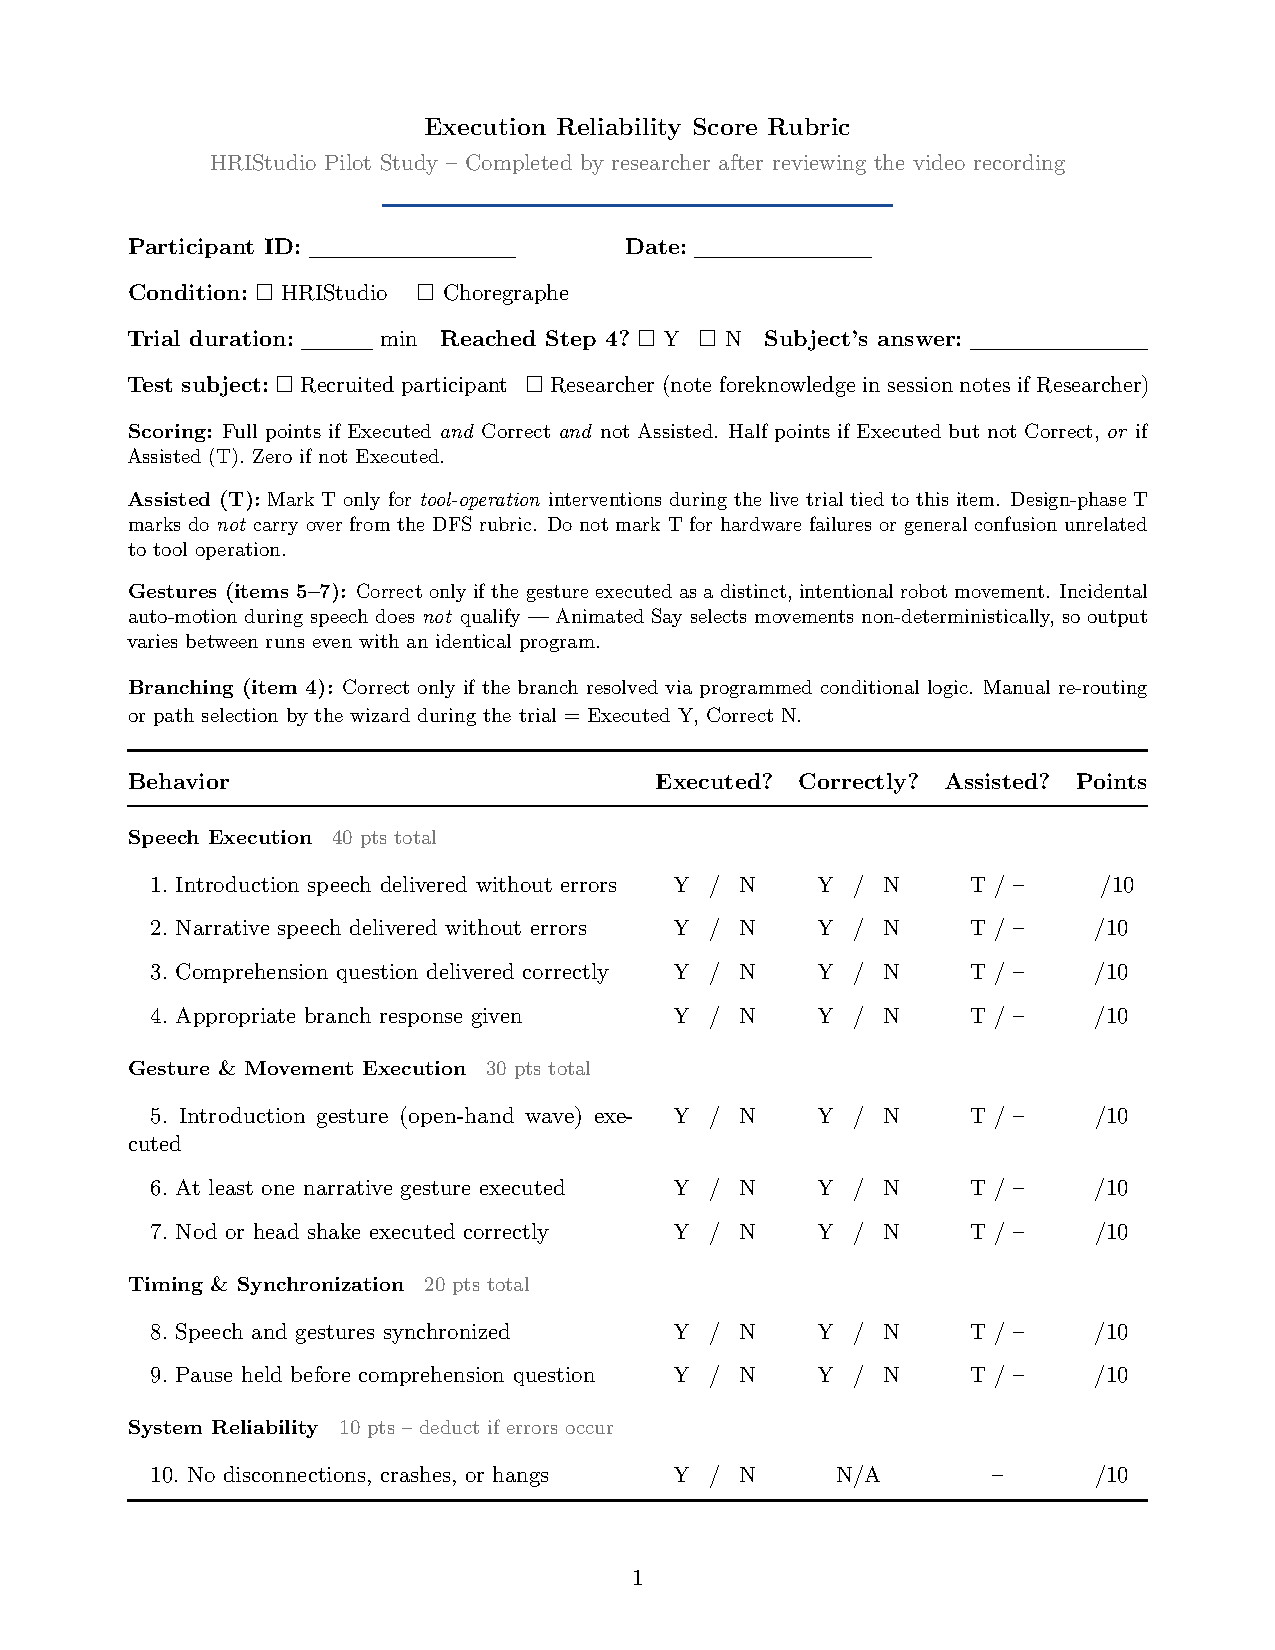
\includepdf[pages=-,pagecommand={}]{pdfs/templates/ERS-Template.pdf}
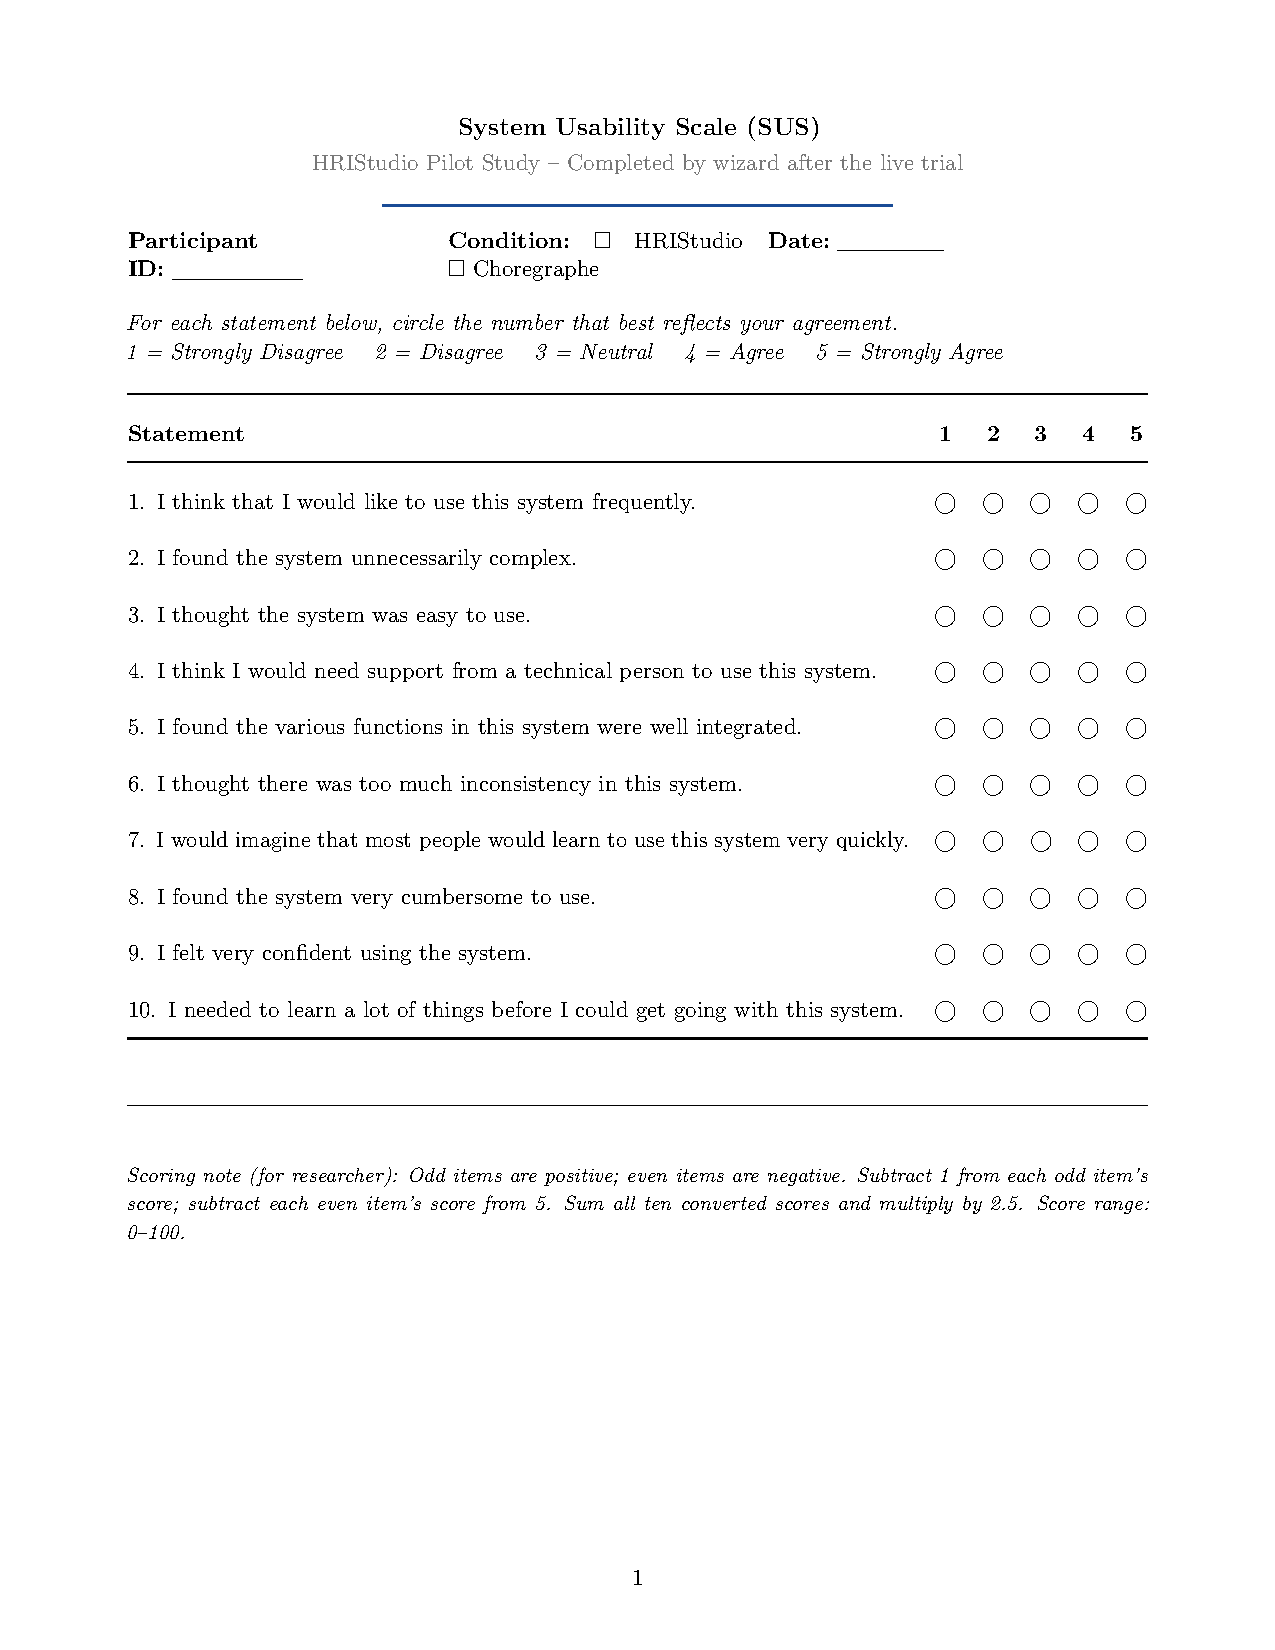
\includepdf[pages=-,pagecommand={}]{pdfs/templates/SUS-Template.pdf}
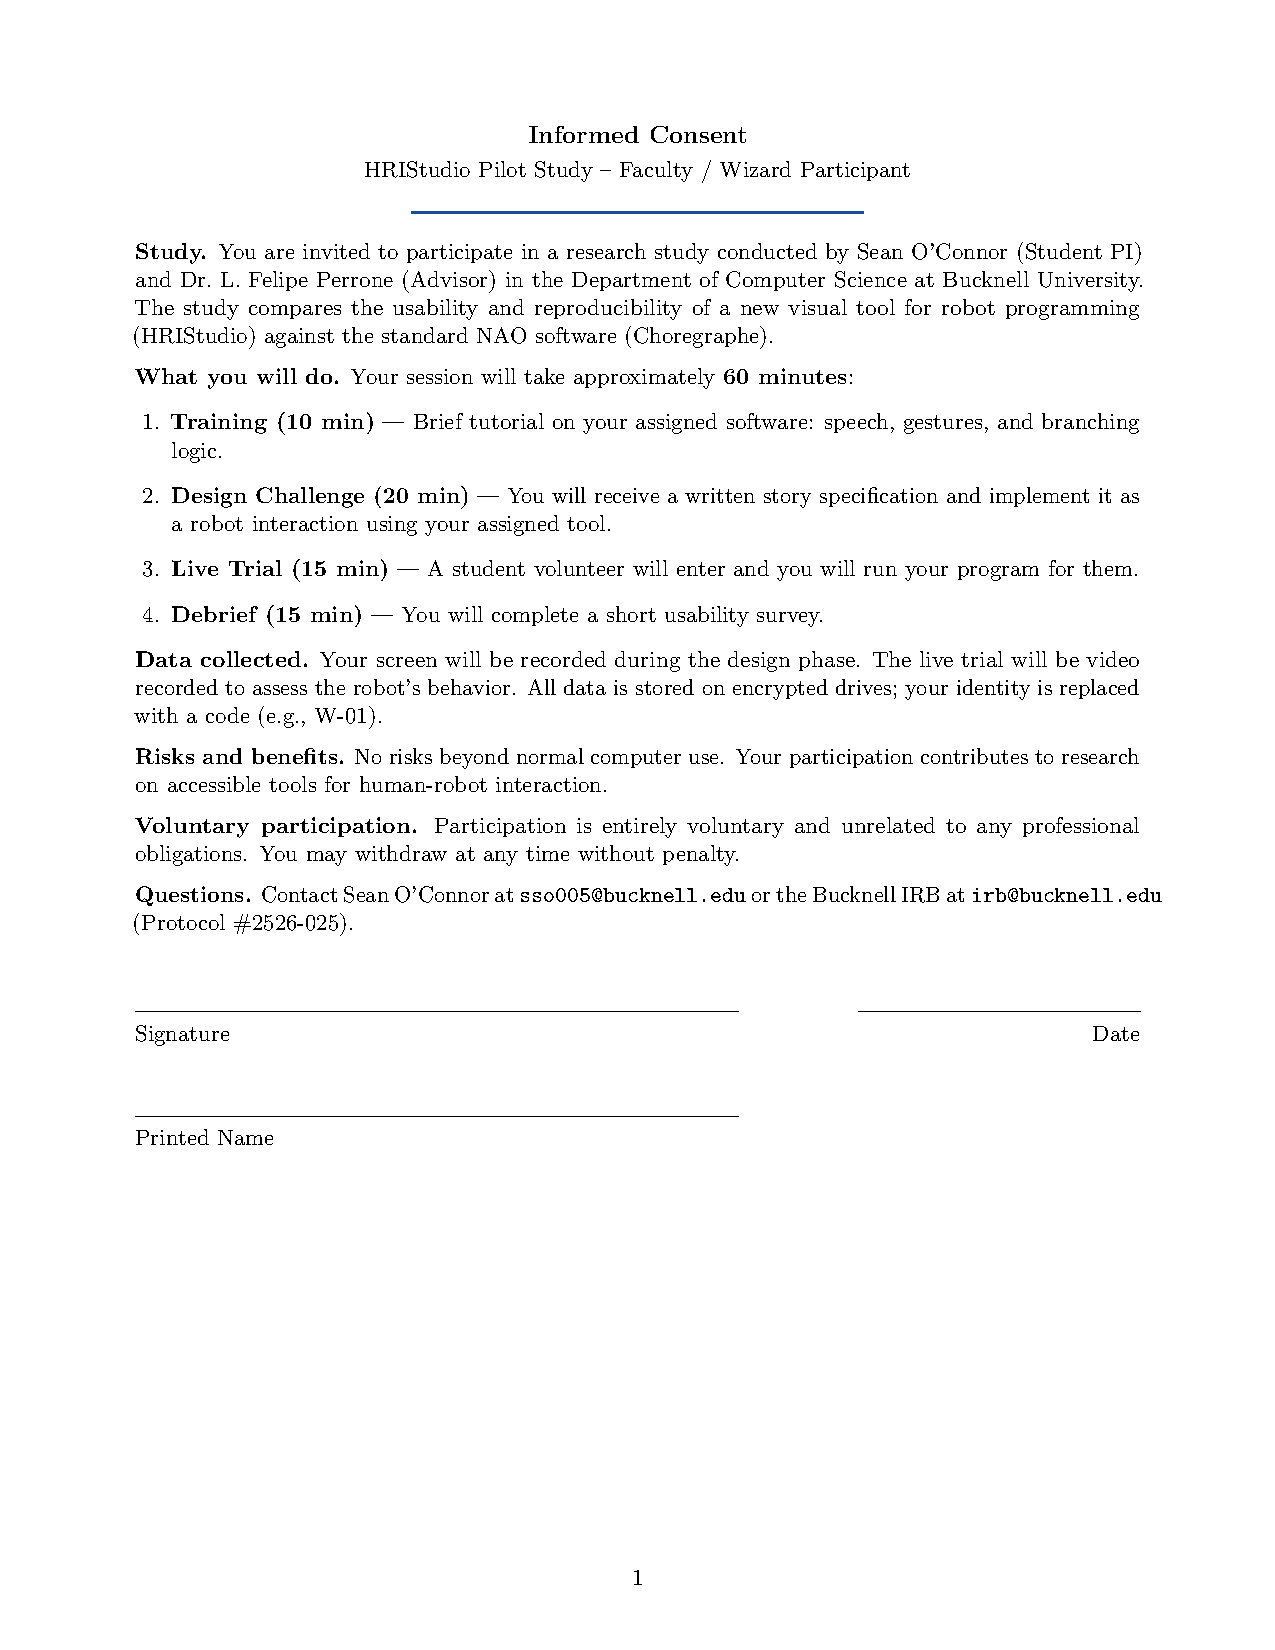
\includepdf[pages=-,pagecommand={}]{pdfs/templates/ICF-Template.pdf}

\chapter{Study Materials}
\label{app:materials}

\textit{[PLACEHOLDER: Study materials will be inserted here. Content includes recruitment materials, paper specification, consent forms, SUS questionnaire, Design Fidelity Score rubric, Execution Reliability Score rubric, observer data sheet, and training protocol.]}

\chapter{Technical Documentation}
\label{app:tech_docs}

This appendix documents the specific technologies and libraries used to build HRIStudio, organized by the three architectural layers described in Chapter~\ref{ch:design}. The goal here is reference, not justification; Chapter~\ref{ch:implementation} explains the reasoning behind the major architectural choices.

\section{Technology Stack}

\subsection{User Interface Layer}

The frontend is built on Next.js (App Router) using React and TypeScript. TypeScript is used throughout the entire codebase, including the server and data access layers, so that type inconsistencies between layers are caught at compile time rather than at runtime. Styling is handled with Tailwind CSS and the shadcn/ui component library. The drag-and-drop canvas in the Design interface uses the \texttt{@dnd-kit} library (\texttt{@dnd-kit/core} and \texttt{@dnd-kit/sortable}) to manage nested drag operations for arranging steps and action blocks.

\subsection{Application Logic Layer}

The server runs as a Next.js Node.js process. API routes use tRPC over HTTP for typed request/response calls; real-time communication during live trials uses a persistent WebSocket connection via the \texttt{ws} package. Authentication and session management are handled by NextAuth.js (v5 beta) with the \texttt{@auth/drizzle-adapter} and bcryptjs for password hashing. Currently, credential-based (username and password) authentication is supported.

\subsection{Data and Robot Control Layer}

Experiment protocols, trial records, and user data are stored in PostgreSQL. The schema and all database queries are managed through Drizzle ORM, which provides compile-time type safety for database interactions. Action configuration parameters and plugin-specific fields are stored as JSONB columns, which allows the same schema to accommodate any robot's action types.

Video and audio recordings captured during trials are stored in a self-hosted MinIO instance, an S3-compatible object storage service. Recordings are captured in the browser using the native MediaRecorder API (assisted by \texttt{react-webcam}) and uploaded to MinIO as a chunked transfer when the trial concludes.

Robot communication is handled through a ROS Bridge (\texttt{rosbridge\_suite} or \texttt{ros2-web-bridge}) running on the robot's local network. The server connects to the bridge over a WebSocket and exchanges JSON-encoded ROS messages; it does not run as a ROS node itself. The bridge address is configured per robot in the plugin file (for example, \texttt{"rosbridgeUrl": "ws://localhost:9090"} in the NAO6 plugin).

\section{Deployment}

The full stack is orchestrated using Docker Compose. The \texttt{docker-compose.yml} file defines three services: the PostgreSQL database (\texttt{postgres:15}), the MinIO storage instance, and the Next.js application server. Starting the entire system on any machine with Docker installed is a single \texttt{docker compose up} command. This configuration is intended for on-premises deployment, which is important for studies involving participant data that cannot leave the institution's network.

\section{Plugin Specification}

Robot capabilities are defined in JSON plugin files. Each file describes a robot platform and the actions it supports. The structure of a plugin file is as follows:

\begin{itemize}
  \item \textbf{Metadata}: name, version, and a human-readable description of the platform.
  \item \textbf{ROS configuration} (\texttt{ros2Config}): the bridge URL and any global connection parameters.
  \item \textbf{Actions}: an array of action definitions. Each action specifies:
    \begin{itemize}
      \item A unique action type identifier (e.g., \texttt{speak}, \texttt{raise\_arm})
      \item A human-readable label shown in the Design interface
      \item A parameter schema defining the input fields the researcher configures
      \item The target ROS topic and message type
      \item A mapping from parameter names to message fields
    \end{itemize}
\end{itemize}

When the server dispatches a robot command, it loads the active plugin, locates the matching action definition, constructs the ROS message by applying the parameter mapping, and sends it to the bridge. Adding a new robot means writing a new plugin file; no server code changes are required.

\section{Role-Based Access Control}

HRIStudio uses a two-layer role system. System roles (\texttt{systemRoleEnum}) govern what a user can do across the platform: \emph{administrator}, \emph{researcher}, \emph{wizard}, and \emph{observer}. Study roles (\texttt{studyMemberRoleEnum}) govern what a user can see and do within a specific study: \emph{owner}, \emph{researcher}, \emph{wizard}, and \emph{observer}. A user's system role and study role are checked independently, so a user who is a wizard on one study can be an observer on another without any additional configuration.


\end{document}
